\documentclass[12pt]{article}

% packages
\usepackage{graphicx}
\usepackage{afterpage}
\usepackage[T1]{fontenc}
\usepackage{afterpage}
\usepackage{amsmath,bm}
\usepackage{amsthm}
\usepackage{parskip}
\usepackage{minted}
\usepackage{amsfonts}
\usepackage[hidelinks]{hyperref}
\usepackage[backend=biber]{biblatex} 
\usepackage{geometry}
\geometry{
a4paper,
total={170mm,257mm},
left=30mm,
right=30mm,
top=30mm,
bottom=30mm,
}

% commands
\newcommand\blankpage{%
    \null%
    \thispagestyle{empty}%
    \addtocounter{page}{-1}%
    \newpage%
}

% cambio del nome alla tabella dei contenuti
\renewcommand*\contentsname{Indice}

% graphic settings
\graphicspath{ {./images/} }

% thm definitions
\theoremstyle{definition}
\newtheorem*{esempio}{Esempio}

% risorse bibliografia (run "biber main" to compile)
\addbibresource{bibliography.bib}

\begin{document}

    % prima pagina
    \begin{titlepage}
    \begin{center}
        
        \includegraphics*[width=0.8\linewidth]{universita_degli_studi_di_genova.png}
        
        \vspace*{0.5cm}

        \textbf{Dipartimento di Informatica, Bioingegneria, Robotica e Ingegneria dei Sistemi}

        \vspace*{0.5cm}

        \textbf{Corso di Laurea Triennale in Informatica}\\
        \textbf{Anno Accademico} 2021/2022

        \vspace*{2cm}
        
        \LARGE
        \textbf{Analisi di serie temporali\\\large Aspetti Applicativi}

        \vspace*{5.5cm}

        \normalsize

        \textit{Candidato}
        \hfill
        \textit{Relatore}\\

        Alex Valle
        \hfill
        Prof.\ Francesca Odone\\

    \end{center}
\end{titlepage}

    % indice
    \tableofcontents

    % introduzione
    \section{Introduzione}
In tale capitolo introduttivo verranno spiegati gli obbiettivi e la suddivisione del tirocinio
in merito al tempo disponibile, cercando di spiegare, in maniera sintetica, come è stato
svolto ed organizzato.

\subsection{Premessa}
Lo scopo di questo elaborato è quello di descrivere l'esperienza di tirocinio svoltasi presso
l'Università Degli Studi di Genova con durata complessiva di 300 ore con inizio 25 novembre 2022
e fine 27 febbraio 2023. Il tirocinio è stato svolto per la maggior parte del tempo da remoto
con incontri, volti all'andamento di esso, mediante l'utilizzo di Teams (piattaforma sviluppata da Microsoft)
che in presenza presso il dipartimento. 

\subsection{Obbiettivi}
L'obbiettivo di questo tirocinio è stato quello di provare a individuare, se esistenti, uno o più metodi, 
relativi all'analisi di serie temporali, che permettano l'analisi di una serie di 
dati relative a soggeti sani e petologici con lo scopo di analizzare il cammino.
\\
I dati utilizzati sono stati analizzati precedentemente da un gruppo di ricerca del dipartimento
con tecniche differenti da quelle utilizzate durante il tirocinio
quindi in caso di un metodo sicuro e soddisfacente all'analisi, i risultati ottenuti sarebbero
serviti al gruppo di ricerca come un'ulteriore conferma delle analisi da loro eseguite.

\subsection{Suddivisione del lavoro}
Per poter garantire la conoscienza necessaria allo sviluppo di un metodo relativo allo scopo
del tirocinio, il lavoro è stato principalmente suddiviso in due fasi: studio dei metodi
relativi all'analisi di serie temporali ed effettivo sviluppo, e ricerca, di un metodo per l'analisi
del problema posto.\\
\\
Nella prima fase sono stati studiati i metodi ed applicazioni di tecniche volte allo studio
di serie temporali, sia da un lato pratico che da un lato teorico. Per quanto riguarda il lato 
pratico, queste tecniche sono state studiante mediante la ricerca di articoli e videotutorial online
sull'applicazione di esse e poi, in una fase successiva, messe in pratica con piccoli esempi 
mediante l'utilizzo di dataset di vario genere, forniti in maniera gratuita da siti web trovati 
su internet, per poterne capire meglio il funzionamento.\\
Per quanto riguarda il lato teorico di esse è stato necessario studiare una piccola base di statistica
inferenziale ed altre nozioni generali per interpretare al meglio i risultati e le tecniche utilizzate in 
ambito applicativo.\\
\\
Nella seconda fase essendo che i dati forniti erano dati ``grezzi'', prima di passare concretamente 
alla ricerca ed implementazione di un metodo volto a risolvere il problema posto, è stato 
necessario applicare in partenza tutte le tecniche di manipolazione dei dati come filtraggio, 
rinomina delle colonne, tecniche per la sostituzione di valori nulli etc \dots per poter 
ottenere un dataset pulito e lavorabile dal punto di vista applicativo. 

    % prima parte del tirocinio
    \section{Studio dei metodi e delle applicazioni}
In tale capitolo verranno spiegati i metodi, le applicazioni ed i concetti 
generali studiati durante la prima fase del tirocinio, accostando ad ogni 
di essi una relativa implementazione e/o utilizzo.\\
In primo luogo si troverà una definizione di serie temporale, seguita da
una spiegazione dei metodi per manipolare i dati inerenti a serie temporali 
su python, le componenti principali di una serie temporale e la loro visualizzazione
ed infine metodi per l'analisi di essi.\\
\\
Molti degli esempi forniti in questa sezione fanno riferimento a dataset disponibili
al sito ``UCI Machine Learning Repository''~\cite{dua:2019} più precisamente, come
esempio, è stato utilizzato un dataset relativo alla qualità dell'aria della città di
Beijing~\cite{dua:air_quality} (Pechino).
 
\subsection{Cos'è una serie temporale}
In statistica descrittiva, una serie storica (o temporale) si definisce come un insieme di variabili 
casuali ordinate rispetto al tempo, ed esprime la dinamica di un certo 
fenomeno nel tempo. Le serie storiche vengono studiate sia per 
interpretare un fenomeno, individuando componenti di trend, di ciclicità, 
di stagionalità e/o di accidentalità, sia per prevedere il suo 
andamento futuro~\cite{wiki:serie_storica}.
In altre parole una serie storica (o temporale) è un'insieme/serie di dati
capionati ed indicizzati nel tempo ad intervalli regolari come ore, giorni 
o anni.\\
\\
In termini più matematici: indichiamo con $\bm{Y}$ il fenomeno (ad esempio 
il prezzo della benzina dall'anno $1970$ all'anno $2010$) ed indichiamo con
$\bm{Y_t}$ un'ossevazione al tempo $\bm{t}$, con $\bm{t}$ un numero intero
compreso tra $\bm{1}$ a $\bm{T}$, dove $\bm{T}$ è il numero totale degli intervalli o 
periodi. Una serie temporale viene espressa in questa maniera 
$\bm{Y_t} = \left\{  \bm{Y_1}, \bm{Y_2}, \dots , \bm{Y_T}  \right\}$.

\begin{esempio} [\textit{Prezzo della benzina}]
    Se consideriamo come fenomeno $\bm{Y}$ il prezzo della benzina dal $1970$ al $2010$
    avremmo come numero totale di osservazioni (o numero totale di periodi) 
    $\bm{T} = \bm{40}$ dove:
    \begin{itemize}
        \setlength\itemsep{-0.5em}
        \item $\bm{Y_1}$: prezzo della benzina all'anno $1970$
        \item $\bm{Y_2}$: prezzo della benzina all'anno $1971$
        \item $\bm{Y_T} = \bm{Y_{40}}$: prezzo della benzina all'anno $2010$
    \end{itemize}

\end{esempio}
    \subsection{Metodi per la gestione dei dati}
In questo sottocapitolo verranno spiegati i metodi studiati ed utilizzati per la gestione dei
dati in python, più nello specifico: come caricare un dataset, una possibile rinomina delle
colonne ralative alle serie per una maggiore comprensione, scelta di un indice, individuazione dei valori
nulli ed infine una sezione relativa al filtraggio.

\paragraph{Cosa viene inteso per dataset} Per dataset si intende un insieme di
serie (nella nostra applicazione temporali) relative ad un'unica applicazione.

\begin{esempio}[\textit{Qualità dell'aria}]
    Consideriamo, per esempio, come applicazione le misurazioni di diversi parametri
    relativi alla qualità dell'aria di Genova: livello di $\mathsf{CO_2}$,
    livello di $\mathsf{SO_2}$, livello di $\mathsf{NO_2}$ e temperatura in \textdegree$\mathsf{C}$.
    In un dataset possiamo considerare ogni parametro come una serie temporale diversa ma indicizzata
    nel tempo in ugual maniera, quindi se queste misurazioni avvengono ogni ora avemo
    per ogni istante di tempo $t$ le misurazioni per ogni parametro in quell'istante.
    \begin{itemize}
        \setlength\itemsep{-0.5em}
        \item $Y_1$: livello di $\mathsf{CO_2}$, $\mathsf{SO_2}$, $\mathsf{NO_2}$ e temperatura in \textdegree$\mathsf{C}$ all'istante $1$.
        \item $Y_2$: livello di $\mathsf{CO_2}$, $\mathsf{SO_2}$, $\mathsf{NO_2}$ e temperatura in \textdegree$\mathsf{C}$ all'istante $2$.
        \item \dots
        \item $Y_T$: livello di $\mathsf{CO_2}$, $\mathsf{SO_2}$, $\mathsf{NO_2}$ e temperatura in \textdegree$\mathsf{C}$ all'istante $T$.
    \end{itemize}
    Ogni parametro in un dataset viene rappresentato come una colonna.
\end{esempio}
Da qusto momento in poi, nel report, quando si parlerà di dataset varrà inteso il tipo
\texttt{pandas.DataFrame}, cioè il modo in cui un dataset viene intrpretato all'interno
di python, mentre per serie si intenderà il tipo \texttt{pandas.Series} oppure un semplice
tipo \texttt{list} di python.

\subsubsection{Pacchetti utilizzati}
Per effettuare tutte le manovre relative all'elaborazione e manipolazione dei dati sono state
utilizzate funzionalità fornite da pacchetti python come \texttt{pandas}, \texttt{numpy} e \texttt{scipy}, essi semplificano
la scrittura di codice e velocizzano il tempo di sviluppo organizzando in maniera ottimale
i dati. Per essere utilizzati essi necessitano prima di essere installati tramite il
gestore di pacchetti di python \texttt{pip}.
\paragraph{Snippet per l'installazione dei pacchetti}
\begin{minted}{bash}
    pip install pandas
    pip install numpy
    pip install scipy
\end{minted}
\paragraph{Snippet per il caricamento in python}
\begin{minted}{python3}
    import pandas as pd
    import numpy as np
    from scipy import signal
\end{minted}



\subsubsection{Caricamento di un dataset}
Per poter utilizzare i dati all'interno di python è stata utilizzata
la funzionalità di pandas \texttt{read\_csv} dove, ogni colonna fa riferimento 
ad una serie.
\paragraph{Snippet}
\begin{minted}{python3}
    dataset = pd.read_csv('data.csv')
\end{minted}





\subsubsection{Rinomina delle colonne relative alle serie}
In qualche case, il primo passo da eseguire, è quello di rinominare
le colonne relative ad ogni serie così da poter avere una rappresentazione
più accurata del dataset.
Tramite l'utilizzo della funzione \texttt{display} e del metodo \texttt{head}
del dataset possiamo controllare i primi $5$ valori di un dataset
controllando anche così il nome di ogni colonna.
\paragraph{Snippet}
\begin{minted}{python3}
    display(dataset.head())
\end{minted}
\begin{figure}[h!]
    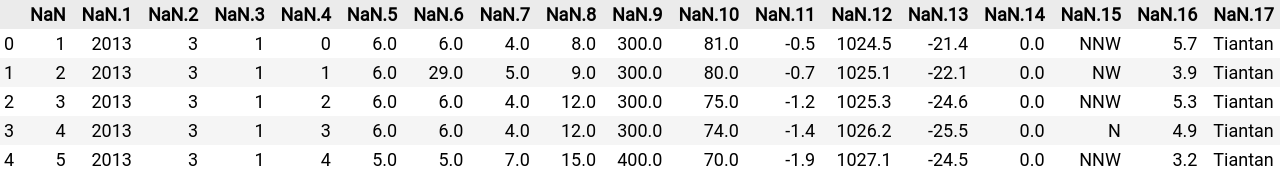
\includegraphics[width=\linewidth,height=2.7cm]{head_before_rename.png}
    \caption{output del metodo head prima della rinomina delle colonne}
    \label{fig:head_before_rename}
\end{figure}
Come si può notare nell'immagine~\ref*{fig:head_before_rename} i nomi delle colonne 
non hanno nessun nome significativo, con il seguente esempio potremmo
cambiare il nome delle colonne.

\paragraph{Snippet}
\begin{minted}{python3}
    # definizione di una lista di nomi per le colonne del dataset
    dataset.columns = [ 'no',    'year',  'month', 'day', 'hour', 
                        'pm2_5', 'pm10',  'so2',   'no2', 'co',  
                        'o3',    'temp',  'pres',  'dewp','rain',  
                        'wd',    'wspm',  'station']
    display(dataset.head())
\end{minted}
\begin{figure}[h!]
    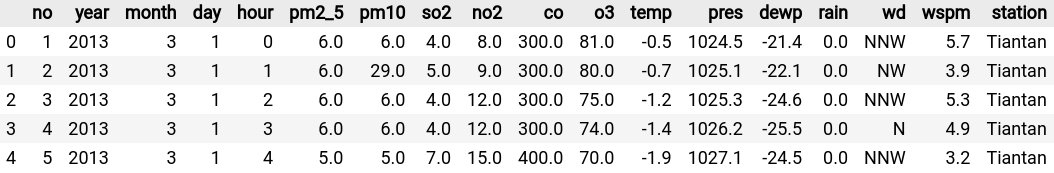
\includegraphics[width=\linewidth,height=2.7cm]{head_after_rename.png}
    \caption{output del metodo head dopo la rinomina delle colonne}
    \label{fig:head_after_rename}
\end{figure}
Come si può notare nell'immagine~\ref*{fig:head_after_rename}
assegnando la lista delle colonne come attuali nomi per le serie del dataset
riusciamo ad ottenere un'interpretazione più accurata.


\subsubsection{Scelta dell'indice}
Molte delle funzionalità fornite da \texttt{pandas} ed altri pacchetti python
richiedono che il dataset sia indicizzato nel tempo nel corretto modo.
In figura~\ref*{fig:head_after_rename} si può notare che la prima colonna
senza nome e la seconda colonna con nome \texttt{no}, indichino
il numero di riga per ogni misurazione, la differenza è che la prima colonna
è generata automaticamente dal pacchetto \texttt{pandas}, ed impostata
di default come indice, mentre la seconda con
nome \texttt{no} è fornita direttamente dal file csv precedentemente caricato.
Per l'analisi della maggior parte delle serie temporali un'idicizzazione per numero
di riga non è significativa, sarebbe molto più conveniente lavorare avendo
come indice di tabella la data ed ora di ogni effettiva misurazione.
A questo proposito il dataset caricato ci fornisce delle colonne (\texttt{year}
, \texttt{month}, \texttt{day} e \texttt{hour}) indicizzate per tempo e relative
ad ogni misurazione, che possono essere riformattate insieme ed usate come indice
per il dataset.

\paragraph{Snippet}
\begin{minted}{python3}
    # unificazione delle colonne relative al tempo per ogni 
    # istante di tempo t in una nuova colonna
    new_index_column = []
    for i in range(len(dataset.year)):
    new_index_column.append("%s/%s/%s %s:0:0" 
        % (dataset.day[i], dataset.month[i], 
           dataset.year[i], dataset.hour[i]) )

    # elimina le colonne relative al tempo
    del dataset["year"], dataset["month"], 
        dataset["day"], dataset["hour"], 
        dataset["no"]

    # imposta/crea la nuova colonna date e converti in datetime
    dataset['date'] = new_index_column
    dataset['date'] = pd.to_datetime(dataset.date, dayfirst=True)

    # imposta come index la nuova colonna date
    dataset.set_index("date", inplace=True)
    display(dataset.head())
\end{minted}
\begin{figure}[h!]
    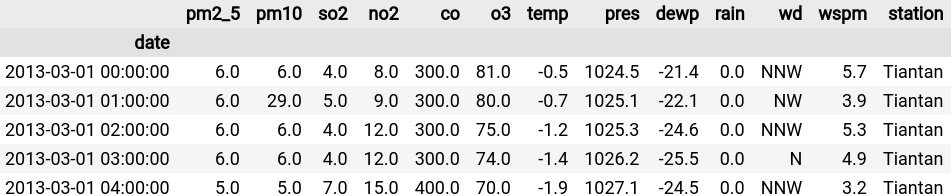
\includegraphics[width=\linewidth,height=2.7cm]{head_after_index_set.png}
    \caption{output del metodo head dopo aver impostato l'indice}
    \label{fig:head_after_index_set}
\end{figure}
Come si può notare dall'output del metodo \texttt{head} nell'immagine \ref*{fig:head_after_index_set}
\texttt{date} è stato impostato come indice di tabella e quindi da questo momento in poi
possiamo accedere al dataset, scegliendo le misurazioni interessate, utilizzando la
data.

\paragraph{Periodo di campionamento}
Un'altra importante modifica è impostare il periodo di campionamento del dataset,
in poche parole impostare un corretto indice non basta a massimizzare il corretto
funzionamento delle funzionalità di analisi delle serie temporali, bisogna anche specificare
l'istante di tempo che occorre tra una misurazione e l'altra. Per fare ciò
\texttt{pandas} fornise un metodo che imposta il periodo di campionamento
a quello deiderato, nel nostro caso sappiamo che le misurazioni sono state campionate
ogni ora.
\subparagraph{Snippet}
\begin{minted}{python3}
    # imposta il periodo di capionamento 
    # del dataset ad ogni ora
    dataset = dataset.asfreq("h")
\end{minted}

\subsubsection{Individuazione dei valori nulli e possibili soluzioni}
La presenza di valori nulli in una serie può avere molteplici cause, ad esempio,
l'impossibilità da parte dello strumento di capionare ad un certo istante di tempo $t$,
oppure se pensiamo ad una fotocamera che acquisisce delle coordinate relative ad un soggeto,
l'uscita di esso dall'obbiettivo.

Indifferentemente dal motivo per cui dei valori nulli sono presenti, 
in una serie o un dataset, la loro presenza può causare molti
problemi sia nel corretto funzionamento di alcune funzionalità per l'analisi sia perchè
non avere dei valori in determinati punti della serie, in certe applicazioni, potrebbe
essere un problema. \texttt{pandas} fornisce dei metodi utili, e semplici, alla soluzione di questo
problema ma ovviamente ogni problema è diverso e quindi, per applicazioni specifiche,
potrebbe essere necessario cercare soluzioni differenti. In questa sezione ci limitiamo
a descrivere le funzionalità fornite da \texttt{pandas} per la soluzione a questo problema.

\paragraph{Controllo}
Per controllare la presenza di valori nulli \texttt{pandas} fornisce un metodo chiamato
\texttt{isna} che ritorna un dataset dove, per ogni misurazione, indica \texttt{True}
se la misurazione è \texttt{NaN} altrimenti \texttt{False}. Sommando i valori \texttt{True}
per ogni colonna possiamo controllare quanti valori nulli sono presenti per ogni serie.\\
\\
\subparagraph*{Snippet}
\begin{minted}{python3}
    # controllo valori nulli
    dataset.isna().sum()
\end{minted}
\begin{figure}[h!]
    \centering
    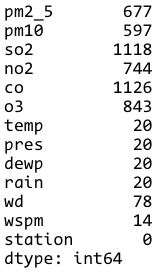
\includegraphics[width=0.24\linewidth,height=5cm]{somma_valori_nulli.png}
    \caption{output della somma dei valori nulli relativi ad ogni serie del dataset}
    \label{fig:sum_null}
\end{figure}
Come si puo notare dall'output del comando in figura~\ref*{fig:sum_null}
il nostro dataset contiene molteplici valori nulli, ora vediamo come poter risolvere
il segente problema

\paragraph{Back fill o Forward fill}
\texttt{pandas} fornisce la possibilità di ``riempire'' i valori nulli in due diverse
modalità tramite l'utilizzo del metodo \texttt{fillna}
\begin{itemize}
    \item \textbf{Back fill}: permette di sostituire i valori nulli con la succesiva
    misurazione valida.
    \item \textbf{Forward fill}:  permette di sostituire i valori nulli propagando
    l'ultima valida misurazione alla prossima valida.
\end{itemize}
Entrambi i metodi gestiscono i valori nulli più o meno nella stessa maniera ma la scelta
di uno piuttosto che l'altro cambia da caso in caso dipendendtemente dal risultato
ottenuto dopo l'utilizzo di essi.


Per i nostri esempi il risulato nell'utilizzo di un metodo piuttosto che l'altro
portava comunque ad un risultato soddisfacente.\\
\\
\subparagraph*{Snippet}
\begin{minted}{python3}
    # rimepimento dei valori nulli 
    # mediante il metodo di forward fill
    dataset = dataset.fillna(method="ffill")
    dataset.isna().sum()
\end{minted}
\begin{figure}[h!]
    \centering
    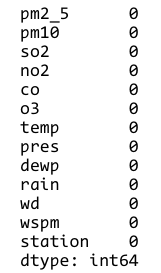
\includegraphics[width=0.24\linewidth,height=5cm]{somma_valori_nulli_dopo_fill.png}
    \caption{output della somma dei valori nulli relativi ad ogni serie del dataset dopo l'utilizzo del metodo \texttt{fillna}.}
\end{figure}


\paragraph{Interpolazione} 
Un possibile metodo, non fornito dalle funzionalità del pacchetto \texttt{pandas},
che potrebbe essere utilizzato è quello di interpolare i dati così da poter colmare
i vuoti creati dai valori nulli. Questa funzionalità non è stata sviluppata
in quanto non fine allo scopo di questo tirocinio ma, in certe applicazioni, si potrebbe
voler utilizzare una metodologia basata su questa tecnica per ottenere una rappresentazione
più accurata dei dati.


\paragraph{Altro metodo non convenzionale}
Un altro metodo non convenzionale, non presente tra le funzionalità fornite,
è quello di poter eliminare i valori nulli dalle serie semplicemente
eliminandoli. Ovviamente questo concetto di eliminare una misurazione nulla va
contro a tutte le premesse fatte fino ad ora, non avendo così una ``reale''
serie temporale poichè mancherebbe una misurazione ad un determinato istante di tempo
$t$, e molte delle analisi che si vorrebbero poter fare su una serie risulterebbero
inapplicabili. 
Tuttavia, in qualche applicazione particolare (come vedremo in seguito), una funzionalità
che semplicemente elimina i valori nulli da una serie potrebbe tornare comoda.
\subparagraph*{Snippet}
\begin{minted}{python3}
    import math as math # import del pacchetto math

    def delete_nan(series: pd.Series | list):
    """ emlimina i valori nulla da una serie
    """
    new_series = []
    for idx, value in enumerate(series):
        if not math.isnan(value):
            new_series.append(value)
    return np.array(new_series)
\end{minted}


\subsubsection{Filtraggio}
Nella maggior parte dei casi quando si parla di serie temporali fonite direttamente 
da apparecchiature che eseguono le misurazioni, i dati si presentano in maniera
``grezza'' ed è quindi necessario filtrarli per poter rimuovere una buona parte
del rumore presente. Questo passaggio è molto importante se parliamo di dati non elaborati
in quanto avere del rumore in una serie temporale o, più in generale, in qualsiasi
tipo di segnale, porta a leggere delle misurazioni ``false''. Solitamente il rumore
indesiderato risiede nelle frequenze alte del segnale, quindi, a questo proposito,
vediamo come poter filtrare una sorgente ``grezza'' di dati mediante l'utilizzo del
modulo \texttt{signal} del pacchetto \texttt{scipy}.

\paragraph{Filtro di Butterworth}
Per poter rimuovere una buona parte del rumore, come scelta generale, in questo tirocinio,
si è utilizzato il filtro di Butterworth che permette di regolare parametri come la 
frequenza di taglio e l'inclinazione (slope) della curva di taglio.

\begin{figure}[H]
    \centering
    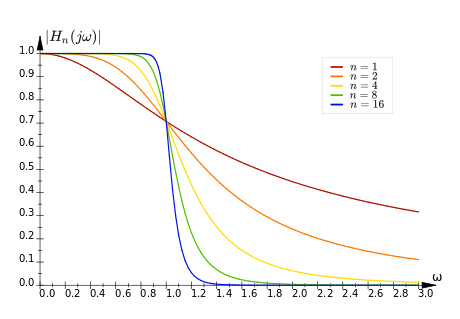
\includegraphics[width=0.7\linewidth,keepaspectratio]{butterworth_filter.png}
    \caption{Filtro di Butterworth normalizzato.}
    \label{fig:butterworth_filter}
\end{figure}

Per poter apprezzare la differenza tra un segnale filtrato da un segnale ``grezzo''
seguirà un esempio su come questo filtro possa essere applicato tramite l'utilizzo
delle funzionalià fornite dal modulo precedentemente citato.

\begin{esempio} [Utilizzo del filtro di Butterworth]
Consideriamo un segnale la cui distanza tra ogni misurazione è di $\frac{1}{30}$
di secondo, presenta una frequenza di campionamento di $30\mathsf{Hz}$.

\begin{figure}[H]
    \centering
    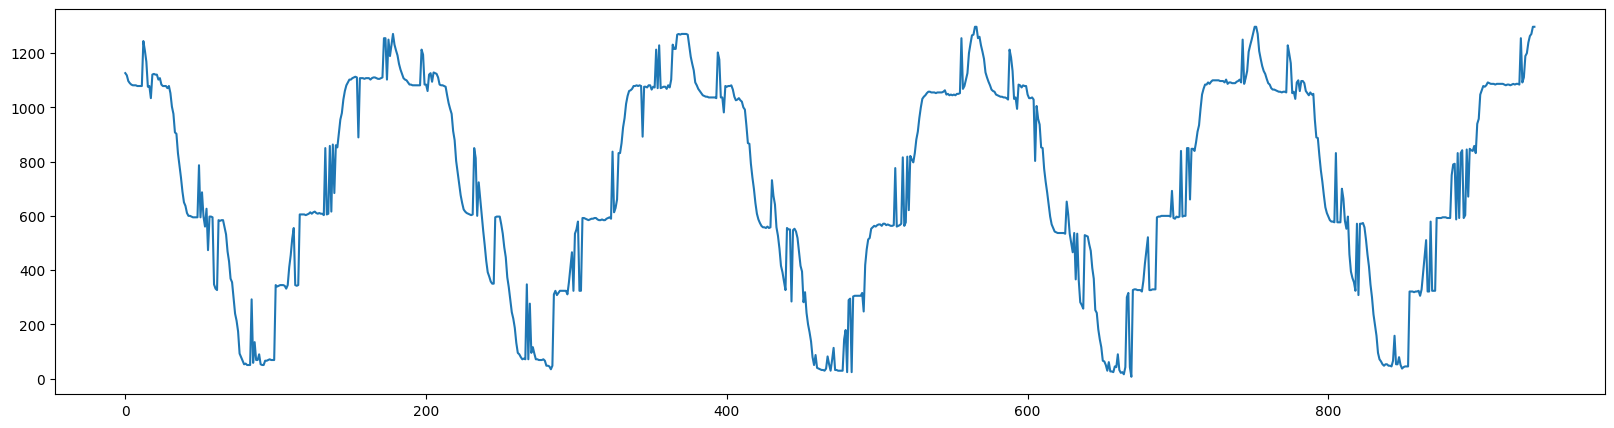
\includegraphics[width=\linewidth,height=4.2cm]{segnale_non_filtrato.png}
    \caption{Segnale non filtrato.}
    \label{fig:segnale_non_filtrato}
\end{figure}

In figura~\ref*{fig:segnale_non_filtrato} possiamo notare come nel segnale
in questione sia presente parecchio rumore, facilmente visibile da tutti i picchi 
presenti nel grafico. Proviamo ad applicare il filtro di Butterworth con una frequenza
di taglio sulle $2\mathsf{Hz}$ ed un'inclinazione della curva di taglio di $5$, lasciando
così passare le basse frequenze.


\paragraph{Snippet}
\begin{minted}{python3}
    # slope/inclinazione della curva di taglio
    inclinazione = 5 

    # frequenza di taglio
    frequenza_taglio = 2

    # frequenza di campionamento
    frequenza_di_campionamento = 30

    # creazizone del filtro di Butterworth
    b, a = signal.butter(inclinazione, 
                        frequenza_taglio, 
                        fs=frequenza_di_campionamento)

    # applicazione del filtro sul segnale
    segnale_filtrato = signal.filtfilt(b, a, series)
\end{minted}

\begin{figure}[H]
    \centering
    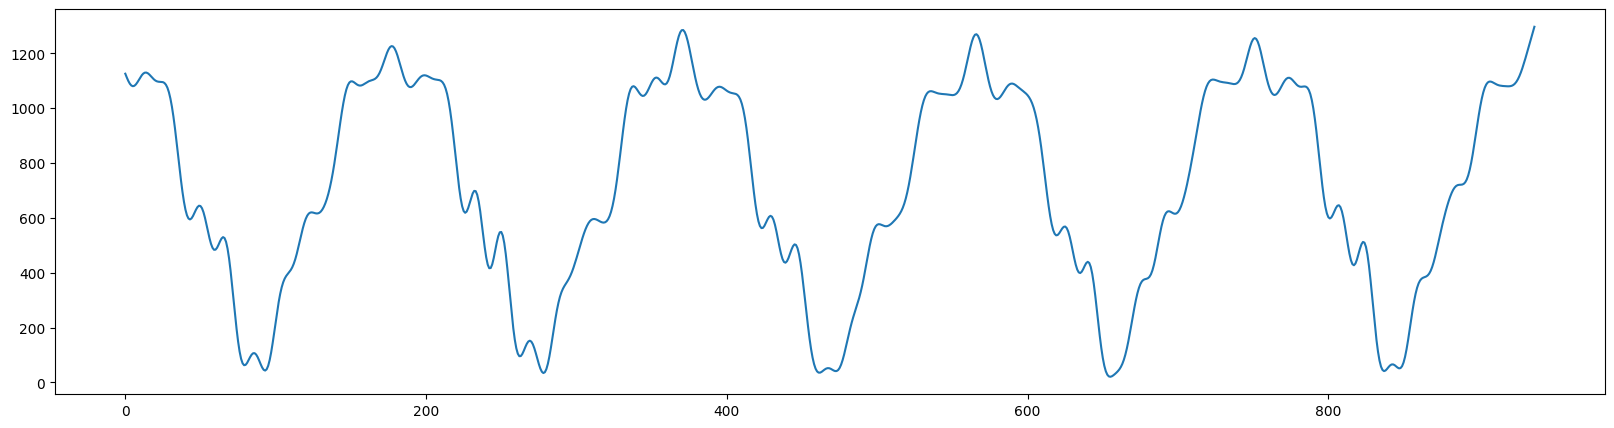
\includegraphics[width=\linewidth,height=4.2cm]{segnale_filtrato.png}
    \caption{Segnale filtrato.}
    \label{fig:segnale_filtrato}
\end{figure}

In figura~\ref*{fig:segnale_filtrato} viene rappresentato il segnale dopo l'applicazione
del filtro passa basse di Butterworth, come si può notare una buona parte del rumore
non è più presente e non avendo i picchi presentati nella sua versione non filtrata.

\end{esempio}


\paragraph{Scelta dei parametri e del filtro}
Dipendendtemente dal tipo di filtraggio che si vuole ottenere conviene applicare un 
filtro piuttosto che un altro e la sua relativa scelta dei parametri cambia da
applicazione ad applicazione e dal tipo di risultato che si vuole ottenere.


    \subsection{Componenti di una serie temporale}
In questo sottocapitolo ci soffermeremo a spiegare le componenti principali
che compongono una serie temporale per poterne analizzare l'andamento e/o
eventuali pattern ricorrenti.


Molte volte è utile suddividere una serie temporale in più diverse componenti
distinte per poterne analizzare singolarmente il loro comportamento e quindi successivamente
riuscire ad inferire sul generale andamento della serie. Possiamo quindi
pensare ad una serie temporale come un insieme di 3 componenti principali:
Trend (andamento/tendenza), Stagionalità e Residui (più comunemente detta Noise).

\subsubsection{Trend}
La componente di trend è un pattern nei dati che mostra che mostra il 
movimento (andamento) di una serie verso valori relativamente più alti o più bassi 
in un lungo periodo di tempo. In altre parole, il trend si osserva quando 
la serie temporale presenta una pendenza crescente o decrescente. 
La tendenza di solito si verifica per un certo periodo di tempo 
e poi scompare, non si ripete. Ad esempio, una nuova canzone, 
che diventa di tendenza per un po' di tempo e poi scompare. 
Non c'è alcuna possibilità che torni in tendenza~\cite{gg:trend}.


Il trend potrebbe essere:
\begin{itemize}
    \setlength\itemsep{-0.6em}
    \item \textbf{Uptrend}: L'analisi delle serie temporali mostra un andamento generale al rialzo, quindi si tratta di Uptrend.
    \item \textbf{Downtrend}: L'analisi delle serie temporali mostra un andamento al ribasso, quindi si tratta di un downtrend.
    \item \textbf{Trend orizzontale o stazionario}: Se non si osserva alcun pattern, si parla di trend orizzontale o stazionario.
\end{itemize}

Se pensiamo al trend come ad una retta, essa sarà la retta che meglio approssima i dati. Se 
la retta ha coefficiente angolare positivo allora essa mostrerà un andamento generale al rialzo,
se ha coefficiente angolare negativo allora essa mostrerà un andamento generale al ribasso, mentre se
avrà coefficiente angolare uguale a $0$ non si osserverà alcun pattern.
Ovviamente nella realtà non sempre una retta basta ad avere una buona approssimazione dei dati, quindi
esistono anche altri tipi di trend come il trend esponenziale.

Nella pratica dell'analisi delle serie temporali in python il trend viene stimato mediante 
l'utilizzo di una funzione chiamata \textit{moving average} (trattata in una sezione successiva).

\begin{esempio} [esempio pratico di trend]
    Consideriamo come serie temporale una serie la cui per ogni osservazione abbiamo
    la temperatura media giornaliera nella città di Beijing a partire 
    dal $01/01/2013$ al $01/01/2017$.

    \begin{figure}[H]
        \centering
        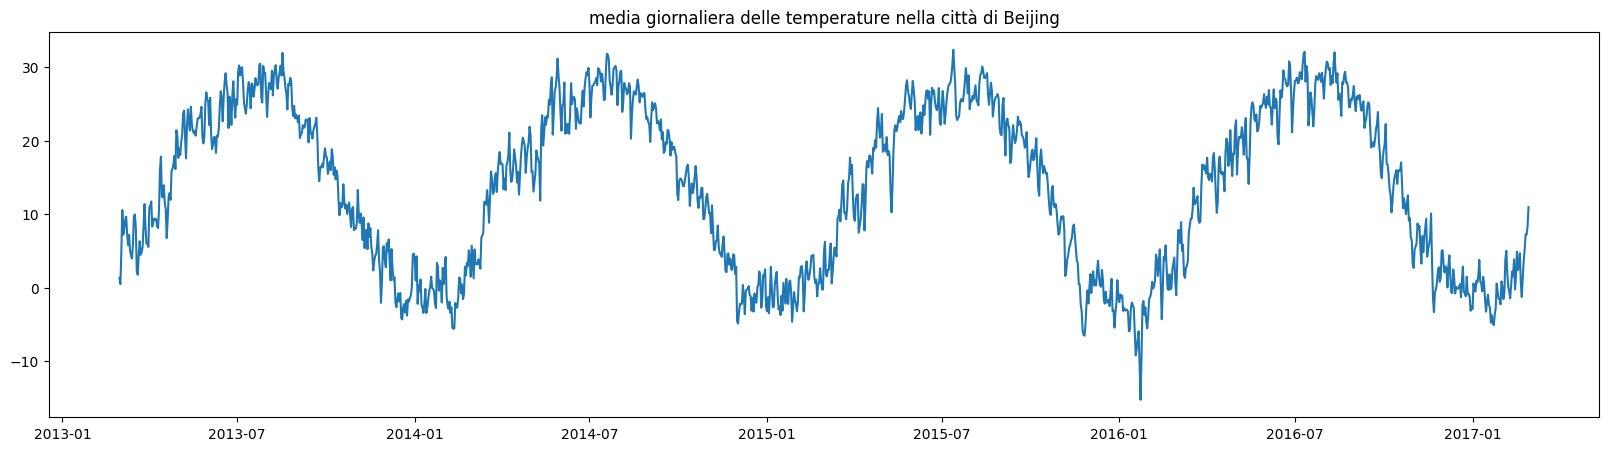
\includegraphics[width=\linewidth,height=4.7cm]{media_giornaliera_temp.png}
        \caption{Grafico della temperatura media giornaliera nella città di Beijing.}
        \label{fig:media_giornaliera_temp}
    \end{figure}

    Consideriamo ora un periodo di un anno ($365$ giorni) il trend avrà un grafico
    come il seguente

    \begin{figure}[H]
        \centering
        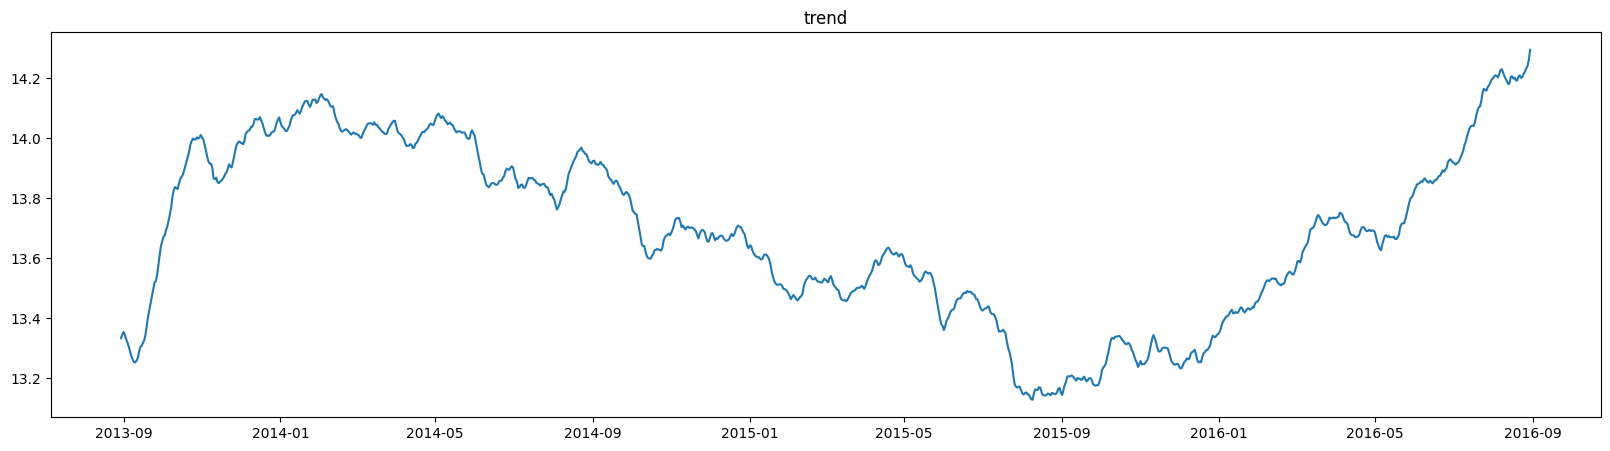
\includegraphics[width=\linewidth,height=4.7cm]{media_giornaliera_temp_trend.png}
        \caption{Trend della serie in figura~\ref{fig:media_giornaliera_temp}.}
        \label{fig:media_giornaliera_temp_trend}
    \end{figure}

    Come possiamo vedere dal grafico in figura~\ref{fig:media_giornaliera_temp_trend} 
    il trend viene stimato utilizzando la media dei precedenti $365$ giorni, ovviamente
    la scelta del periodo su cui stimare il trend influisce direttamente sul grafico. 

\end{esempio}


\subsubsection{Stagionalità}
La stagionalità è un aspetto cruciale dell'analisi delle serie temporali. 
Poiché le serie temporali sono indicizzate in avanti nel tempo, sono soggette a 
fluttuazioni stagionali. Ad esempio, ci aspettiamo che le vendite di gelati siano 
maggiori nei mesi estivi e minori in quelli invernali.

La stagionalità può manifestarsi in diversi intervalli di tempo, 
come giorni, settimane o mesi. La chiave per l'analisi delle serie temporali 
è capire come la stagionalità influisce sulle nostre serie~\cite{md:seasonality}.

In sintesi possiamo quindi pensare alla stagionalità come un pattern che si ripete ad 
intervalli/periodi specifici nel tempo.


\begin{esempio} [esempio pratico di stagionalità]

    Se consideriamo come serie temporale la stessa serie utilizzata 
    nell'esempio precedente del trend, quindi una serie la cui 
    ogni osservazione indica la temperatura media giornaliera  
    nella città di Beijing a partire dal $01/01/2013$ al $01/01/2017$

    \begin{figure}[H]
        \centering
        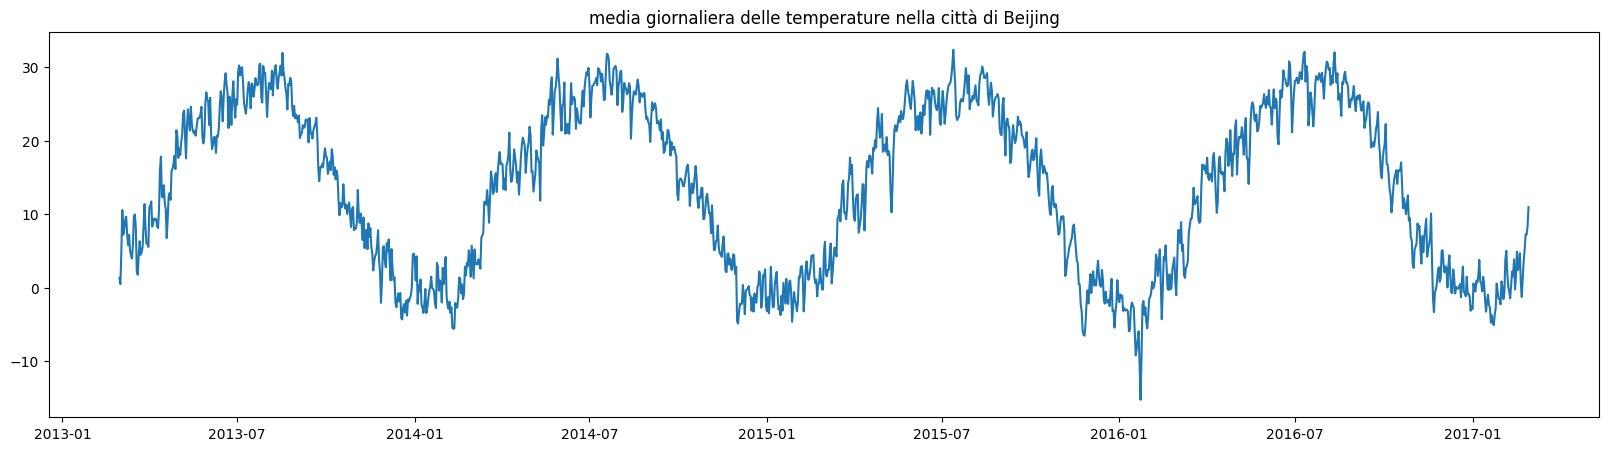
\includegraphics[width=\linewidth,height=4.7cm]{media_giornaliera_temp.png}
        \caption{Grafico della temperatura media giornaliera nella città di Beijing.}
        \label{fig:media_giornaliera_temp2}
    \end{figure}

    e consideriamo un periodo di un anno ($365$ giorni) la stagionalità avrà un grafico
    come il seguente

    \begin{figure}[H]
        \centering
        \includegraphics[width=\linewidth,height=4.7cm]{media_giornaliera_temp_stagionalità.png}
        \caption{Stagionalità del grafico in figura~\ref{fig:media_giornaliera_temp2}.}
        \label{fig:media_giornaliera_temp_stag}
    \end{figure}

    Il grafico in figura~\ref{fig:media_giornaliera_temp_stag} rappresenta la stagionalità
    della serie rappresentata in figura~\ref{fig:media_giornaliera_temp2}.
    Se guardiamo con occhio attento il grafico della stagionalità, possiamo notare come
    ad intervalli di un anno esso si ripeta, creando così il pattern stagionale.

\end{esempio}


\subsubsection{Residui}
La componente di residui, o più comunemente detta noise, può essere considerata come
la parte restante tra il trend e la stagionalità, quindi una sorta di errore.

Un metodo per poter capire meglio come rappresenta la componente di residui 
è considerare, ad esempio, una serie temporale con trend orizzontale e nessun pattern
stagionale, ed applicare la definizione di residui, quindi tutto quello che rimane
tolto il trend e la stagionalità.

\begin{esempio} [esempio pratico di stagionalità]

    Se consideriamo la serie temporale utilizzata negli esempi del trend
    e della stagionalità, la componente dei residui avrà un grafico come il seguente

    \begin{figure}[H]
        \centering
        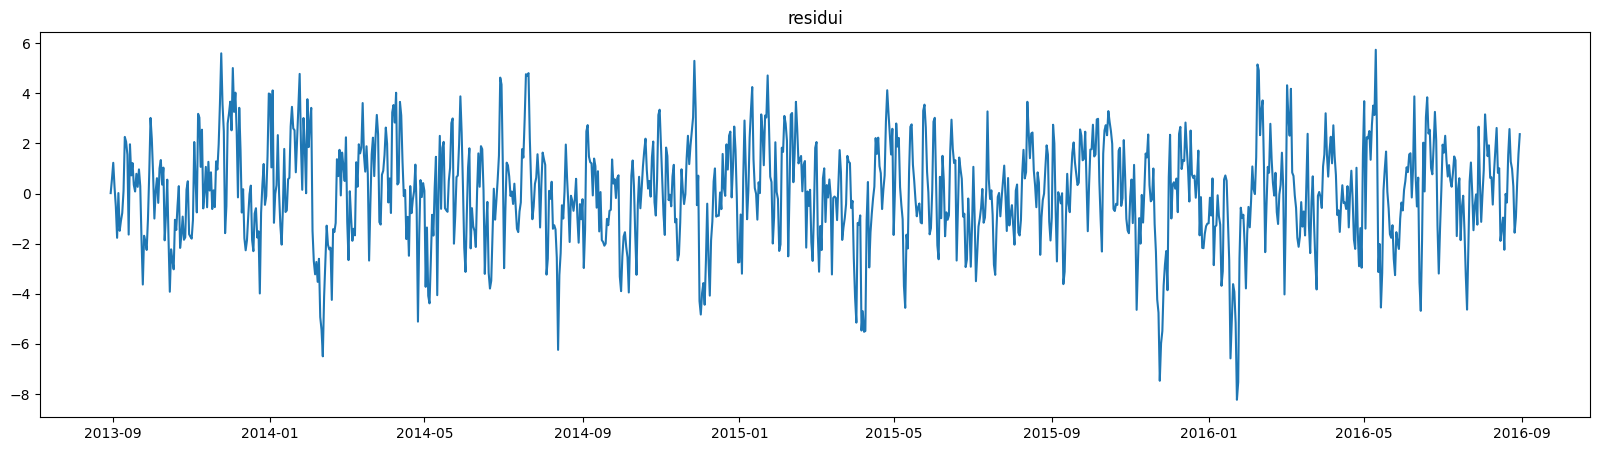
\includegraphics[width=\linewidth,height=4cm]{media_giornaliera_temp_residui.png}
        \caption{Residui della media giornaliera delle temperature nella città di Beijing.}
    \end{figure}

\end{esempio}


\subsubsection{Decomposizione di una serie}
Esistono due modalità distinte per la decomposizione di
una serie temporale nelle sue 3 componenti principali. La prima modalità è detta
additiva in cui le componenti vengono semplicemente sommate, mentre la seconda
è detta moltiplicativa dove le componenti, come suggerisce il termine, 
vengono moltiplicate.

\paragraph{Decomposizione additiva} 
Una decomposizione additiva consiste nella
somma delle componenti. Se consideriamo una serie temporale ad un 
istante $t$ allora essa sarà composta da
\[ y_t = S_t + T_t + R_t \]
dove $y_t$ è l'osservazione, $S_t$ è la componente di stagionalità, 
$T_t$ è la componente di Trend ed $R_t$ è la componente dei residui, tutti
all'istante di tempo $t$.
\begin{figure}[H]
    \centering
    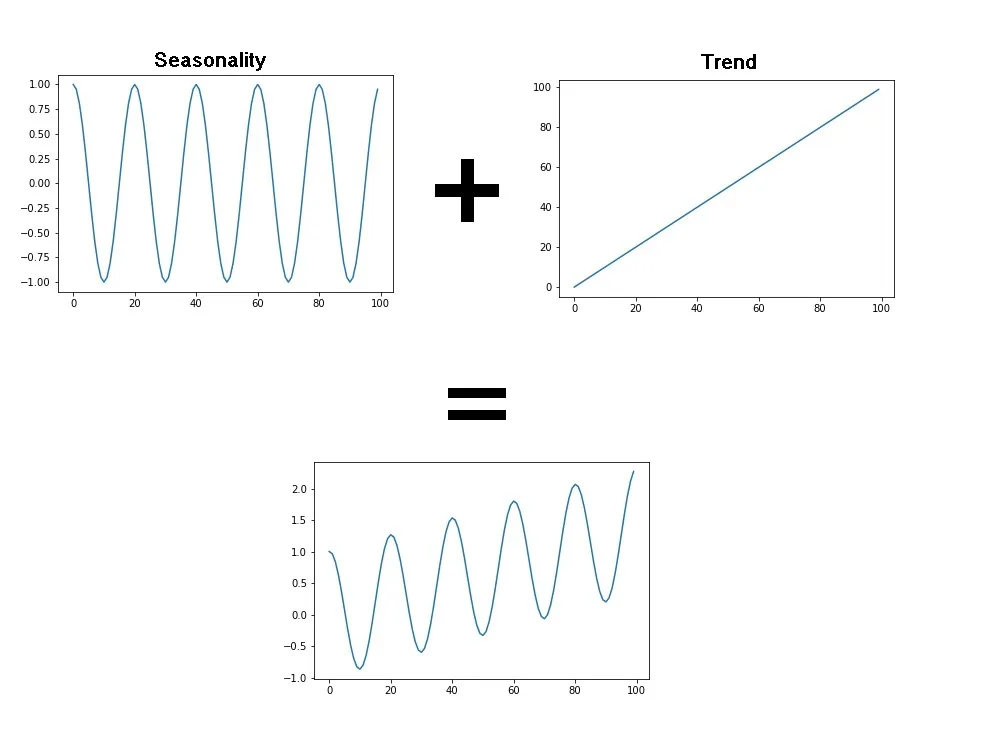
\includegraphics[width=0.6\linewidth]{additive_decomposition.jpg}
    \caption{Decomposizione additiva (escluso residui). [ref imag~\cite{md:seas_dec_imags}]}
    \label{fig:dec_serie_add}
\end{figure}


\paragraph{Decomposizione moltiplicativa} 
Una decomposizione moltiplicativa consiste nella
moltiplicazione delle componenti. Se consideriamo una serie temporale ad un 
istante $t$ allora essa sarà composta da
\[ y_t = S_t \times T_t \times R_t \]
dove $y_t$ è l'osservazione, $S_t$ è la componente di stagionalità, 
$T_t$ è la componente di Trend ed $R_t$ è la componente dei residui, tutti
all'istante di tempo $t$.
\begin{figure}[H]
    \centering
    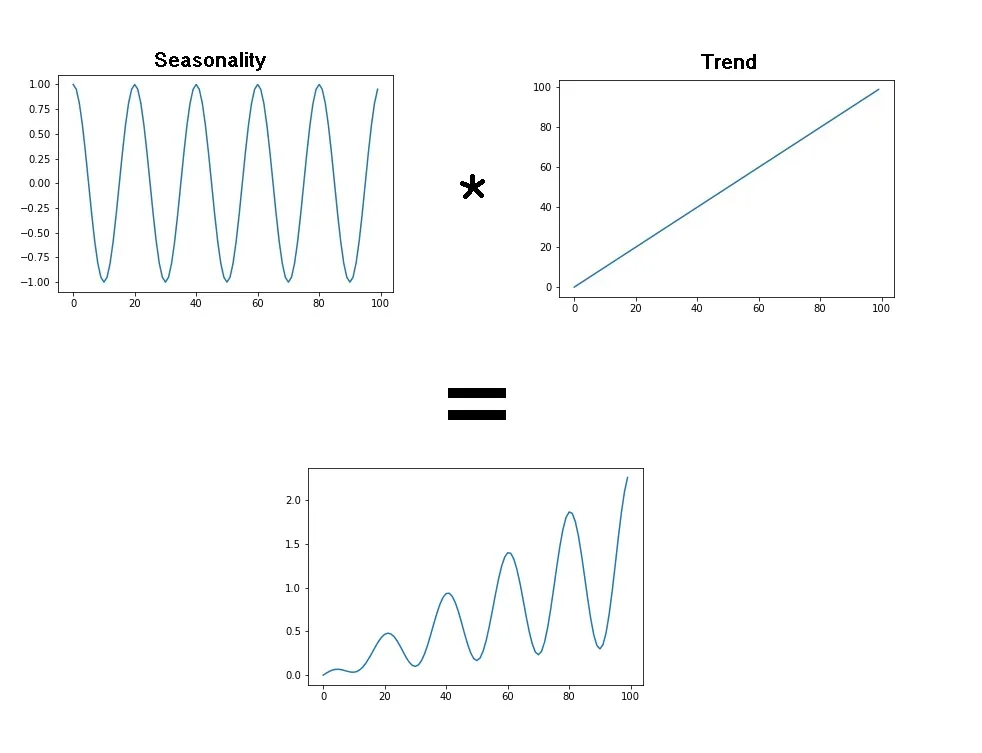
\includegraphics[width=0.6\linewidth]{multiplicative_decomposition.jpg}
    \caption{Decomposizione moltiplicativa (escluso residui). [ref imag~\cite{md:seas_dec_imags}]}
    \label{fig:dec_serie_mul}
\end{figure}

\paragraph{Scelta della modalità di decomposizione}
La scelta della modalità di decomposizione di una serie temporale è importate poiché
la sua decomposizione potrebbe apparire insensata scelta la modalità sbagliata.
Una decomposizione additiva è principalmente appropriata se il magnitudo della 
stagionalità non varia con il livello della serie temporale mentre se, la variazione
della componente di stagionalità, appare proporzionale al livello della serie una modalità
moltiplicativa potrebbe essere più appropriata (per capire la seguente frase guarda le figure
~\ref{fig:dec_serie_add} e~\ref{fig:dec_serie_mul}).


\paragraph{Decomposizione in python}
Vediamo ora come poter decomporre una serie temporale utilizzando la funzione 
\texttt{seasonal\_decompose} fornita dalle funzionalità del pacchetto \texttt{statsmodels}.
\subparagraph*{Installazione del pacchetto}
\begin{minted}{bash}
    pip install statsmodels



\end{minted}

\subparagraph*{Snippet}
\begin{minted}{python3}
    # import del pacchetto 
    from statsmodels.tsa.seasonal import seasonal_decompose

    # periodo utilizzato per il calcolo di trend e stagionalità
    periodo = 365 

    # decomposizione della serie
    decomposition = seasonal_decompose(serie, period=periodo)

    trend   = decomposition.trend     # trend
    stag    = decomposition.seasonal  # stagionalità
    residui = decomposition.resid     # residui
\end{minted}
    \subsection{Stazionarietà}


\subsubsection{Dickey Fuller Test}
    \subsection{Smoothing}

\subsubsection{Moving average}

\subsubsection{Exponential}

\subsubsection{Double Exponential}
    \subsection{Autocorrelazione ed Autocorrelazione parziale}
In questa sezione verranno presentate le funzioni di autocorrelazione ed autocorrelazione
parziale utilizzate nell'analisi di serie temporali per poter trovare pattern e la correlazione
diretta o indiretta della serie con una sua versione spostata lungo l'asse temporale.

Nota che per molte applicazioni (come l'analisi di pattern) che utilizzano le funzioni
di autocorrelazione ed autocorrelazione parziale, le serie temporali devono essere stazionarie.

\subsubsection{Funzione di Autocorrelazione}
L'autocorrelazione definisce il grado di dipendenza tra i valori assunti 
da una funzione campionata nel suo dominio in ascissa. \\
Se è dimostrata l'autocorrelazione tra due valori, al cambiare delle peculiarità 
di uno di essi varierà anche l'altro.

L'autocorrelazione è uno strumento matematico usato frequentemente nella teoria dei 
segnali per l'analisi di funzioni o di serie di valori. Essa è la correlazione 
del segnale (o più in generale del valore di una variabile) con se stesso; 
in altre parole il segnale all'istante di tempo $t$ viene confrontato con un altro valore 
di se stesso ritardato di una quantità 
$\tau$  (senza tale ritardo il segnale è logicamente sempre uguale) 
per verificare quanto si somigli (più precisamente quanto si correli) 
all'avanzare del tempo. Possiamo dedurre che se un segnale varia lentamente nel tempo, 
il valore degli istanti $y(t)$ e $y(t + \tau)$ sarà pressoché simile 
(l'autocorrelazione avrà segno positivo), mentre se varia rapidamente, 
il valore di tali istanti sarà molto diverso e l'autocorrelazione assume 
un valore prossimo allo zero. 
L'autocorrelazione si utilizza spesso per cercare porzioni periodiche che si ripetono 
all'interno di un segnale, in modo tale da determinare la presenza di un segnale 
periodico che è stato sepolto da un rumore, o identificare la frequenza fondamentale 
di un segnale~\cite{wiki:autcor_it}.

Informalmente, è la somiglianza tra le osservazioni di una variabile casuale 
in funzione dell'intervallo di tempo che le separa~\cite{wiki:autcor_en}.

\paragraph{Definizione matematica} 
\subparagraph*{Caso continuo}
Dato un segnale $f(t)$ continuo ed indicizzato nel tempo, l'autocorrelazione $R_{ff}(\tau)$
è definita come la cross-correlazione di $f(t)$ con se stesso avente un ritardo di $\tau$
\[R_{ff}(\tau) = \int_{-\infty}^{\infty} f(t+\tau) \overline{f(t)}  \,dt =  \int_{-\infty}^{\infty} f(t) \overline{f(t-\tau)}  \,dt \]
dove $\overline{f(t)}$ indica il complesso coniugato fi $f(t)$. 
Nota come il parametro $t$ nell'integrale è una variabile fittizia ed è solo necessaria
a calcolare l'integrale. Non ha un significato specifico~\cite{wiki:autcor_en}.

\subparagraph*{Caso discreto}
Nel caso discreto la funzione di autocorrelazione è definita come:
\[ R_{ff}(\tau) = \mathbb{E} \left[ f(t) \overline{f(t-\tau)} \right] = \mathbb{E} \left[ f(t + \tau) \overline{f(t)} \right] \] 

\subparagraph*{Normalizzazione del caso discreto}
La normalizzazione della funzione di autocorrelazione nel caso discreto ci fornisce la 
possibilità di avere una visualizzazione con valori compresi tra $[-1, 1]$. 
Sottraendo la media prima della moltiplicazione si ottiene la funzione di autocovarianza 
\[ 
K_{ff}(\tau) = 
\mathbb{E} \left[ \left( f(t + \tau) - \mu \right) \overline{ \left( f(t) - \mu \right) } \right] =  
\mathbb{E} \left[ f(t + \tau) \overline{ f(t) } \right] - \mu\overline{\mu} 
\] 
dove $\mu$ è la media.


La funzione di autocorrelazione normalizzata viene definita come 

\[ 
\rho_{ff}(\tau) = \frac{K_{ff}(\tau)}{\sigma^2} = 
\frac{\mathbb{E} \left[ \left( f(t + \tau) - \mu \right) \overline{ \left( f(t) - \mu \right) } \right]}{\sigma^2}
\] 



\paragraph{Implementazione della funzione di autocorrelazione ed esempi}
Vediamo ora come poter implementare la funzione di autocorrelazione (normalizzata).
\subparagraph*{Snippet} (\textit{shift di una funzione})
\begin{minted}{python3}
def shift(X, n):
    """ Shifta di n periodi la funzione X
    """


    # controllo per n
    if not isinstance(n, int):
        raise Exception('n deve essere un valore intero')

    X_copy = X.copy() # copia e rendi numpy array
    if not isinstance(X_copy, np.ndarray):
        X_copy = np.array(X_copy)

    # se si shifta troppo impostiamo n
    # alla lunghezza della funzione X
    if np.abs(n) > len(X):
        n = np.sign(n) * len(X)
    
    # dato  n shiftiamo la funzione verso sinistra
    # dato -n shiftiamo la funzione verso destra
    for i in range(np.abs(n)):
        # togliamo il primo o lultimo valore
        # in base a dove vogliamo shiftare
        X_copy = X_copy[1:] if np.sign(n) == 1 else X_copy[:-1]

        # shifta la funzione aggiungendo uno 
        # 0 in testa o in coda in base a dove
        # vogliamo shiftare
        X_copy = np.insert(X_copy, 0 if np.sign(n) == -1 
            else len(X_copy), 0)

    return X_copy.tolist() if not isinstance(X, np.ndarray) \
        else np.array(X_copy)
\end{minted}

\subparagraph*{Snippet} (\textit{singola autocorrelazione})
\begin{minted}{python3}
    def singola_autocorrelazione(X: list | np.ndarray, 
    tau: int, normalizzazione = True) -> float:

    """ Esegue una signola autocorrelazione data la latenza
        tau
    """

    # controllo per tau
    if not isinstance(tau, int) and tau < 0:
        raise Exception('tau deve essere un intero \
            maggiore di 0')

    # controllo che X sia un array numpy
    if not isinstance(X, np.ndarray):
        X = np.array(X)


    if normalizzazione:
        mean = X.mean()
        var = X.var()
        
        # f(t-tau) - mu
        primo_termine   = shift(X - mean, -tau)

        # coniugato(f(t)- mu)
        secondo_termine = np.conjugate(X - mean)

        #                                           ... / sigma^2
        return np.mean( primo_termine * secondo_termine ) / var

    # espettazione[ f(t-tau)       * coniugato(f(t)) ]   
    return np.mean( shift(X, -tau) * np.conjugate(X) )
\end{minted}

\subparagraph*{Snippet} (\textit{funzione di autocorrelazione})
\begin{minted}{python3}
def funzione_autocorrelazione(
    X: list | np.ndarray,
    norm = True
    ) -> list | np.ndarray:
    
    """ calcola la funzione di autocorrelazione
    """
    autocorrelazione: list = []
    # calcola la autocorrelazione singola per ogni
    # possibile tau
    for i in range(len(X)):
        autocorrelazione.append(
            singola_autocorrelazione(X, i, 
                normalizzazione=norm)
        )

    return autocorrelazione if not isinstance(X, np.ndarray) \
        else np.array(autocorrelazione)
\end{minted}

\begin{esempio}[Autocorrelazione]
    Prendiamo come esepio un segnale la cui velocità cambia di ``poco''
    nel tempo.

    \begin{figure}[H]
        \centering
        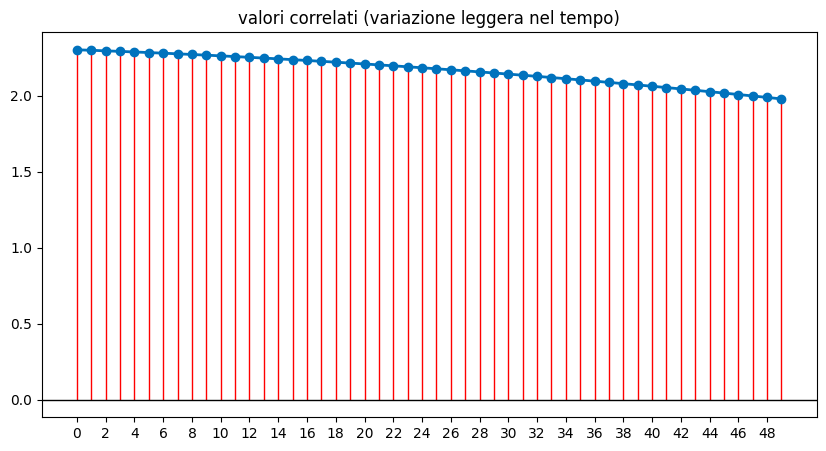
\includegraphics[width=0.9\linewidth,keepaspectratio]{autocor_vel_lenta.png}
        \caption{Autocorrelazione del segnale.}
        \label{fig:autcor_slow}
    \end{figure}

    In figura~\ref{fig:autcor_slow} possiamo notare come l'autocorrelazione non normalizzata
    del segnale varia di poco nel tempo per segnali che variano lentamente.

    Consideriamo ora più segnali la cui velocità cresce velocemente nel tempo.

    \begin{figure}[H]
        \centering
        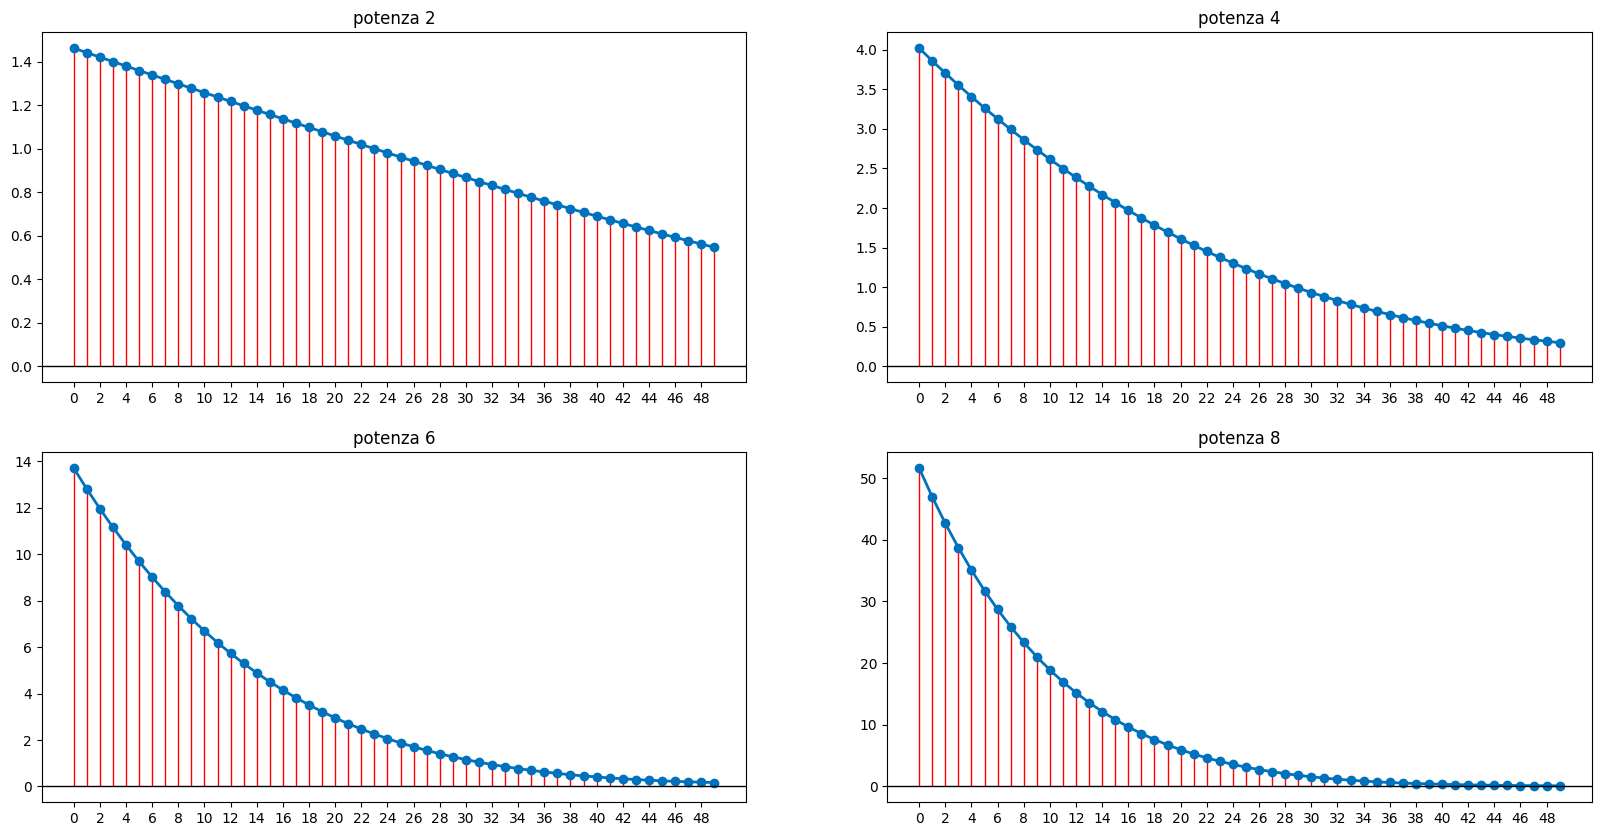
\includegraphics[width=\linewidth,height=9cm]{autocor_vel_fast.png}
        \caption{Autocorrelazione dei segnali.}
        \label{fig:autcor_fast}
    \end{figure}

    In figura~\ref{fig:autcor_fast} possiamo notare come l'autocorrelazione non normalizzata
    dei segnai varia maggiormente nel tempo per segnali che variano velocemente.

    Possiamo quindi osservare come segnali con minima variazione nel tempo avranno anche
    una minima variazione nell'autocorrelazione non normalizzata, mentre segnali che hanno
    un'ampia variazione tra un'osservazione e quella successiva avranno una maggiore variazione 
    anche nell'autocorrelazione non normalizzata.

    Un'ulteriore osservazione che nasce dagli esempi sopra è che i segnali più 
    correlati tra loro sono i segnali con una variazione minore nel tempo, mentre
    i segnali meno correlati saranno i segnali con una maggior variazione. 

\end{esempio}


\subsubsection{Funzione di Autocorrelazione Parziale}
L'autocorrelazione parziale, riassume la relazione tra 
un'osservazione di una serie temporale e le osservazioni di fasi temporali precedenti,
come la normale autocorrelazione con la diversità che le relazioni 
delle osservazioni intermedie vengono rimosse. In sostanza, 
le correlazioni indirette vengono eliminate lasciando visibile solamente
l'effetto diretto~\cite{md:mediumacf_pacf}.

Potreste, ad esempio, essere interessati alla relazione diretta tra i consumi 
di oggi e quelli di un anno fa. Non vi importa nulla di ciò che accade nel mezzo.

Il consumo dei 12 mesi precedenti ha un effetto sul consumo degli 11 mesi precedenti 
e il ciclo continua fino al periodo più recente. Nelle stime di autocorrelazione parziale, 
questi effetti indiretti vengono ignorati~\cite{ain:acf_pacf}.

\paragraph{Calcolo della funzione di autocorrelazione parziale}
La funzione di autocorrelazione parziale teorica di una serie temporale 
stazionaria può essere calcolata utilizzando l'algoritmo di Durbin-Levinson:
\[ \phi_{n,n} = 
\frac
{\rho(n) - \sum_{k = 1}^{n-1}  \phi_{n-1,k}\rho(n-k)}
{1 - \sum_{k = 1}^{n-1} \phi_{n-1,k}\rho(k)} 
\]
    
dove $\phi_{n,k} = \phi_{n-1,k} - \phi_{n,n}\phi_{n-1,n-k}$ per $1 \leq k \leq n-1$ and
$\rho(n)$ è la funzione di autocorrelazione~\cite{wiki:pacf}.

\paragraph{Quando è utile l'autocorrelazione parziale}
La funzione di autocorrelazione parziale gioca un ruolo molto importante, nell'analisi
di serie temporali, per l'identificazione dei lag ``importanti'' per un modello autoregressivo
(AR). Essendo che lo scopo del tirocinio è analizzare 
serie temporali senza eseguire nessuna predizione sui dati con modelli autoregressivi, non verrà
data un'iplementazione della formula presente sopra.

\paragraph{Pacchetto per l'utilizzo}
La funzione \texttt{pacf}, del modulo\\ \texttt{statsmodels.tsa.stattools}, e la funzione
\texttt{plot\_pacf}, del modulo\\ \texttt{statsmodels.graphics.tsaplots}, forniscono rispettivamente
un'implementazione della funzione di autocorrelazione parziale ed il grafico di essa.



    

    % seconda parte del tirocinio
    \section{Gestione dei dataset forniti}
Da questa sezione in poi il tirocinio entrò nella sua seconda fase di durata 1 mese e le succesive
sezioni e sottosezioni, inclusa la medesima, saranno in ordine cronologico di lavoro.

L'obbiettivo di questa sezione è spiegare le scelte applicative che sono state attuate
per l'elaborazione dei dataset e descriverne il loro contenuto, per 
riuscirne a capire le analisi, le soluzioni ed i risultati ottenuti nelle seguenti sezioni. 




\subsection{Descrizione dei dataset}
Durante il tirocinio sono stati forniti più dataset.
Ogni dataset era relativo ad un soggetto, sano o patologico, con una specifica camminata,
più nel dettaglio i dataset erano relativi a camminate normali, sulle punte o tacco punta.
Ogni dataset era formato da più serie temporali, quindi indicizzate nel tempo, relative
alla posizione di un particolare giunto (esempio: piede destro, piede sinistro, naso \dots)

\paragraph{Campionamento dei dati} I dati relativi ad ogni dataset sono stati ottenuti girando un video del soggetto in posizione
laterale e lasciato camminare, avanti ed indietro per un corridoio, davanti all'obiettivo della telecamera. 
Successivamente, i video registrati, sono stati analizzati utilizzando una libreria open source che, con un algoritmo
di machine learning, riconosce i punti relativi alle giunture interessate. Per ogni frame del video
è stato quindi possibile fornire la posizione dei giunti in pixel, sia sull'asse delle
ascisse che delle ordinate, in riferimento al pixel $(0,0)$ del frame analizzato.

Il campionamento dati e la successiva trasformazione di essi in dataset, contenenti le posizioni
dei giunti di ogni soggetto, è stata svolta dal gruppo di ricerca del dipartimento che successivamente
ci ha fornito i dataset elaborati.


\begin{esempio}[Giuntura del naso]
    Se per esempio prendiamo la giuntura del naso relativa ad uno dei dataset, indifferentemente
    dal fatto che esso sia relativo ad un soggetto sano o patologico, essa presenta nel dataset una serie
    chiamata \texttt{x\_naso} e \texttt{y\_naso} che rappresentano rispettivamente 
    la posizione $x$ ed $y$ ad ogni frame acquisito dal video.
\end{esempio}

\subparagraph*{Frequenza di campionamento}
La fotocamera utilizzata per registrare i video ha una frequenza di campionamento di 
$30\mathsf{Hz}$, quindi ogni misurazione è distante dalla successiva circa $33,3\mathsf{ms}$.
Detto ciò la fotocamera riuscirà a captare periodicità che avvengono al massimo ogni $66,6\mathsf{ms}$
($15\mathsf{Hz}$), logicamente per sapere quando un certo evento inizia e finisce abbiamo
bisogno di almeno $2$ misurazioni, più che sufficienti a captare periodicità che risultino
significative all'analisi del movimento di un soggetto.

\subparagraph*{Descrizione delle serie relative ad un dataset}
I giunti forniti dai dataset sono: naso, torace, spalla destra, gomito destro, polso destro, 
spalla sinistra, gomito sinistro, polso sinistro, cresta iliaca, anca destra, ginocchio destro, 
caviglia destra, anca sinistra, ginocchio sinistro, caviglia sinistra, occhio destro, 
occhio sinistro, zigomo destro, zigomo sinistro, piede sinistro ($3$ posizioni), 
piede destro ($3$ posizioni).\\
Per ognuno di questi giunti è presente una misura della posizione sull'asse delle ascisse, 
una misura della posizione sull'asse delle ordinate ed una misura di likelihood cioè un numero
tra $0$ ed $1$ che esprime quanto siamo sicuri di aver trovato il giunto nella posizione giusta
(questa misurazione è stata ignorata).

\subsection{Rinomina delle colonne dei dataset}
I dataset sono stati forniti sprovvisti di una rappresentazione significativa per ogni colonna
quindi, come prima operazione, sono state ridenominate tutte le colonne.

Senza scendere troppo nei dettagli implementativi di come questa operazione è stata eseguita,
poichè una tecnica per la ridenominazione delle colonne è stato fornita nella sezione precedente,
vediamo come i dataset si presentano prima e dopo l'applicazione di essa.

\begin{figure}[H]
    \centering
    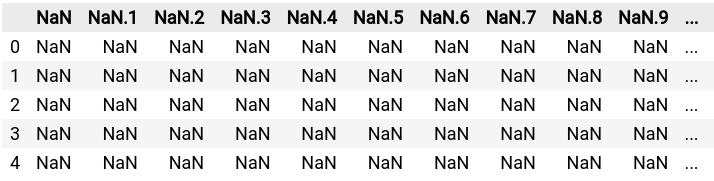
\includegraphics[width=\linewidth,height=2.5cm]{dataset_prima_rinomina.png}
    \caption{Dataset prima della ridenominazione delle colonne.}
    \label{fig:ds_prima_rinomina}
\end{figure}

\begin{figure}[H]
    \centering
    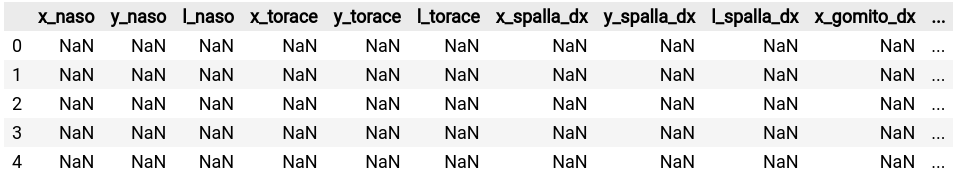
\includegraphics[width=\linewidth,keepaspectratio]{dataset_dopo_rinomina.png}
    \caption{Dataset dopo la ridenominazione delle colonne.}
    \label{fig:ds_dopo_rinomina}
\end{figure}

Come possiamo notare dalle figure~\ref*{fig:ds_prima_rinomina} e~\ref*{fig:ds_dopo_rinomina}
i nomi delle colonne dei dataset sono state ridenominate, esse ora rappresentano meglio
la realtà ed il loro accesso su python facilitato in è possibile accedervi utilizzando
il comando \texttt{dataset\_name.nome\_giunto} invece che \texttt{dataset\_name['nome\_giunto']}.



\subsection{Gestione dei valori nulli}
Nei dataset forniti erano presenti dei valori nulli causati
dall'uscita del soggetto dall'obbiettivo e quindi l'impossibilità, da parte dell'algoritmo
di machine learning, di ottenere una posizione per i giunti interessati.

Essendo che l'obbiettivo finale del tirocinio non è quello di eseguire delle predizioni
sulle serie temporali ma quello di inferire sui dati utilizzando le tecniche
dell'analisi di serie temporali, i valori nulli sono stati semplicemente eliminati.
In questa maniera consideriamo consecutivi dati che effettivamente non lo sarebbero
ma questo non è stato un problema nelle succesive analisi poichè la maggior parte dei 
valori nulli era presente nei momenti in cui il soggetto si girava per eseguire un'ulteriore
camminata davanti all'obiettivo.

Guardiamo ora una esempio di serie prima e dopo l'eliminazione dei valori nulli così da avere
un'idea di come i dati si presentano.

\begin{figure}[H]
    \centering
    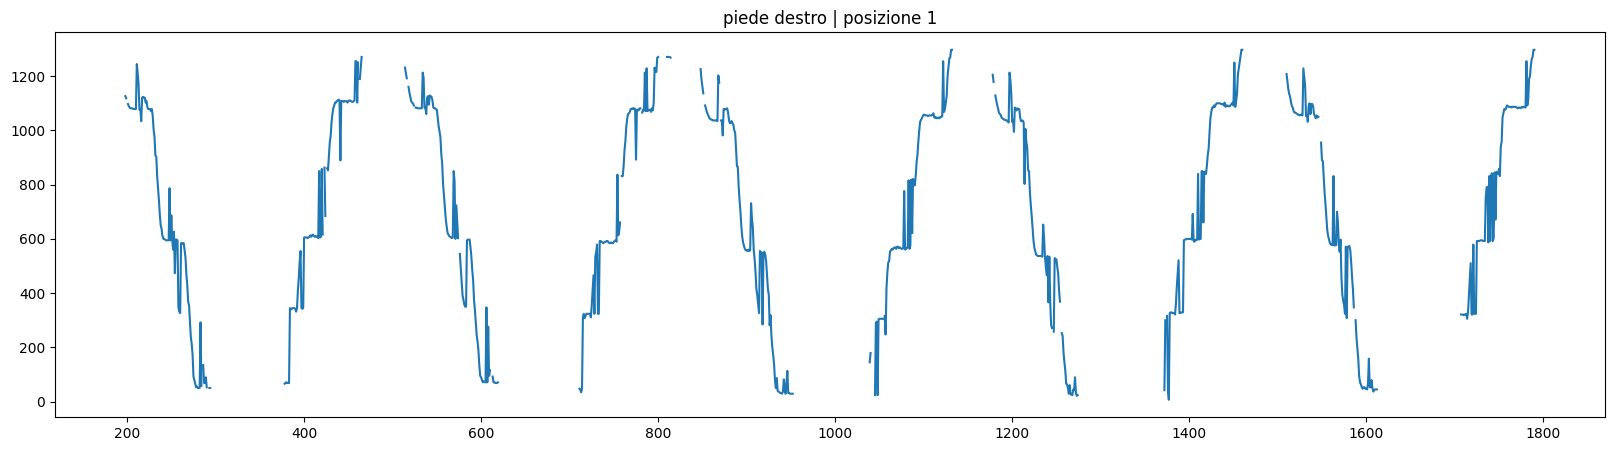
\includegraphics[width=\linewidth,height=4.7cm]{piede_dx_nan.png}
    \caption{Piede destro posizione $1$ con valori nulli.}
    \label{fig:piede_dx_1_nan}
\end{figure}

\begin{figure}[H]
    \centering
    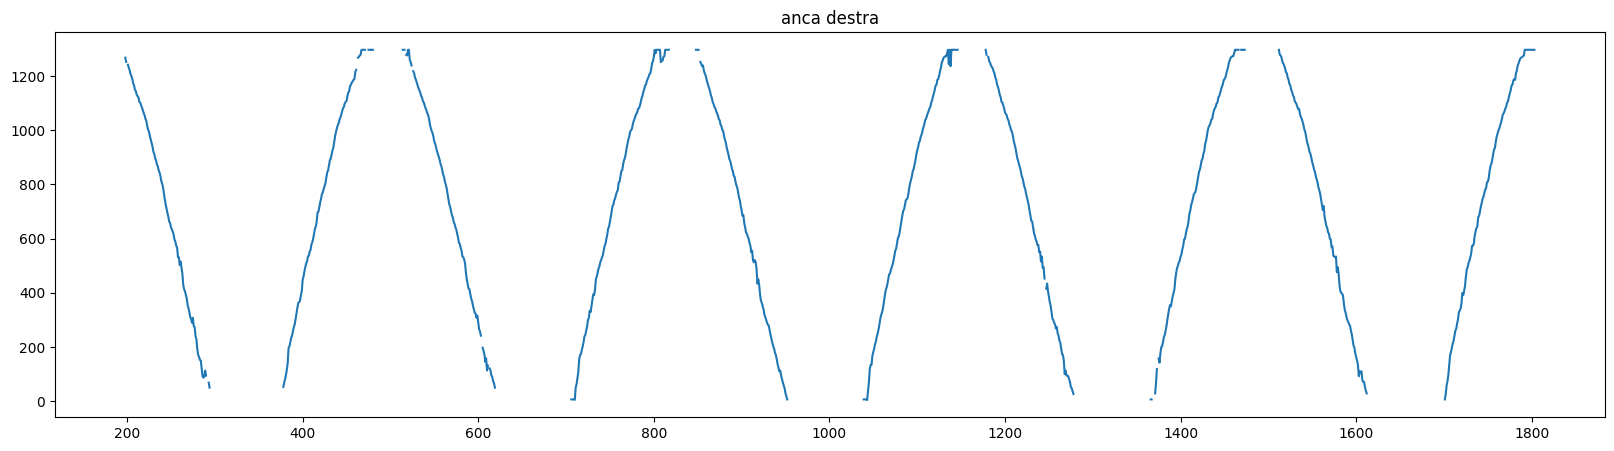
\includegraphics[width=\linewidth,height=4.7cm]{anca_dx_nan.png}
    \caption{Anca destra con valori nulli.}
    \label{fig:anca_dx_nan}
\end{figure}

Come possiamo notare dai grafici in figura~\ref*{fig:piede_dx_1_nan} e~\ref*{fig:anca_dx_nan}
le serie contengono valori nulli nei punti in cui il soggetto esce dall'obiettivo girandosi
per un'altra camminata davanti all'obiettivo.

\begin{figure}[H]
    \centering
    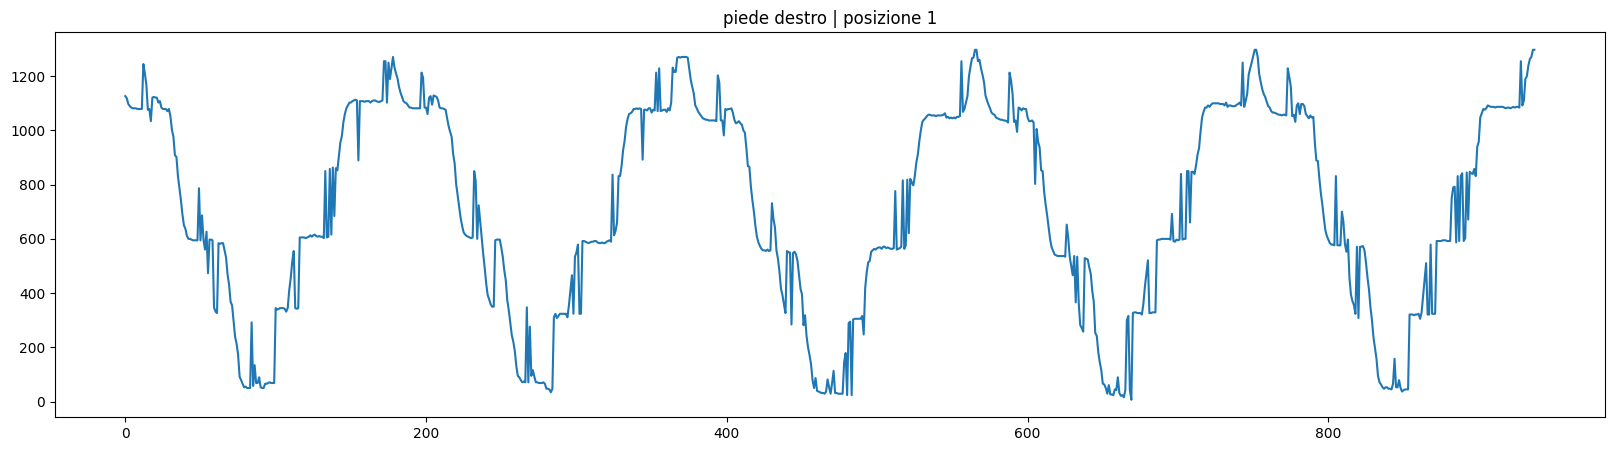
\includegraphics[width=\linewidth,height=4.7cm]{piede_dx_no_nan.png}
    \caption{Piede destro posizione $1$ senza valori nulli.}
    \label{fig:piede_dx_1_no_nan}
\end{figure}

\begin{figure}[H]
    \centering
    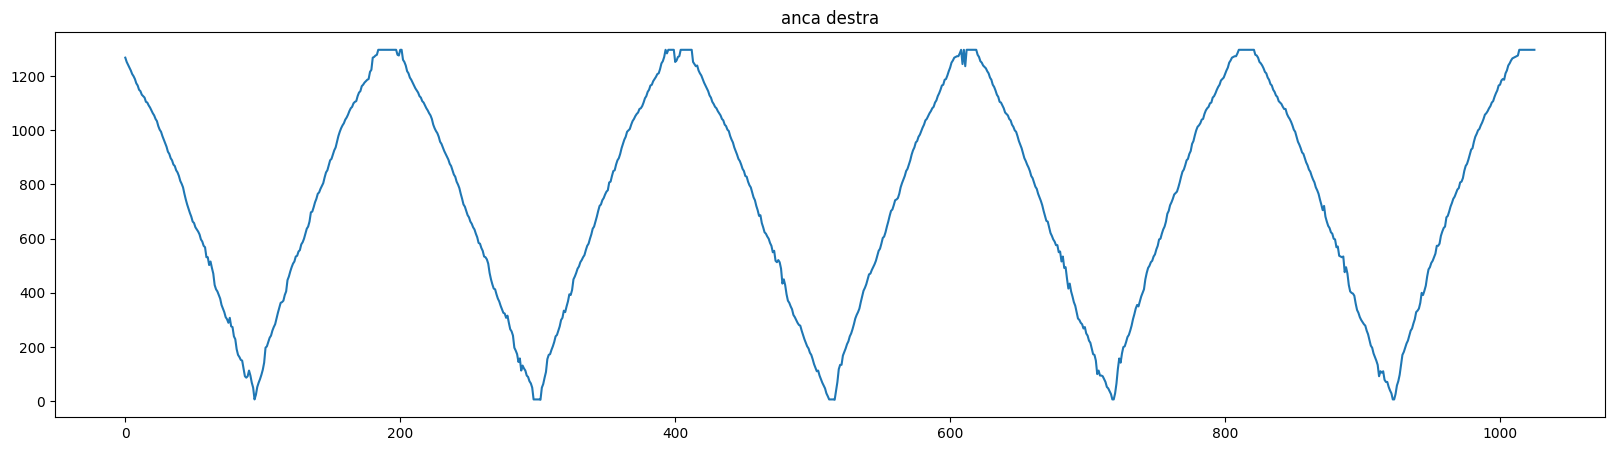
\includegraphics[width=\linewidth,height=4.7cm]{anca_dx_no_nan.png}
    \caption{Anca destra senza valori nulli.}
    \label{fig:anca_dx_no_nan}
\end{figure}

Guardando i grafici rappresentati in figura~\ref*{fig:piede_dx_1_no_nan} e~\ref*{fig:anca_dx_no_nan}
possiamo notare come i valori nulli sono stati eliminati considerando così ogni camminata 
davanti all'obiettivo continua.


\subsection{Scelta dell'indice di tabella per ogni dataset}
Un'osservazione che nasce spontanea dall'osservazione dei grafici in figura
~\ref*{fig:piede_dx_1_nan},~\ref*{fig:anca_dx_nan},~\ref*{fig:piede_dx_1_no_nan}
e~\ref*{fig:anca_dx_no_nan} e dalle tabelle in figura~\ref*{fig:ds_prima_rinomina}
e~\ref*{fig:ds_dopo_rinomina} è che i dataset non sono indicizzati nel tempo utilizzando
la classica indicizzazione come \texttt{anno/mese/giorno ora:minuti:secondi} ma sono indicizzati
in base al frame di acquisizione quindi al numero di riga della tabella.
Questo non è un problema dal punto di vista dell'analisi di ogni serie poichè noto il frame
di acquisizione e la frequenza di campionamento si riuscirà facilmente a risalire ai secodni.

Nel nostro caso, sapendo che i dati sono stati acquisiti con una frequenza di campionamento di 
$30\mathsf{Hz}$, e presa una qualsiasi misurazione ad un certo frame risaliremo al secondo
di tempo con la seguente formula
\[ S_\texttt{frame} = \frac{\texttt{frame}}{30} \]
dove $S_f$ sono i secondi trascorsi dal frame $0$ al frame $\texttt{frame}$ e $\texttt{frame}$ 
è il numero del frame interessato.


\subsection{Filtraggio dei dataset}
Come si può notare dai grafici in figura~\ref*{fig:piede_dx_1_nan},~\ref*{fig:anca_dx_nan},~\ref*{fig:piede_dx_1_no_nan}
e~\ref*{fig:anca_dx_no_nan} le serie dei dataset contengono molto rumore causato da una sbagliata 
lettura della posizione, di ogni giunto, da parte dell'algoritmo di machine learning.

Come spiegato nella precedente sottosezione sul filtraggio, il rumore risiede principalemente nelle
alte frequenze di un segnale.

In linea teorica si è pensato che tutte le frequenze più alte di $2\mathsf{Hz}$ possano essere rumore,
quindi in sostanza si andranno ad eliminare tutte le periodicità e movimenti periodici 
che avvengono sotto $0.5 \mathsf{secondi}$. 

Una soluzione migliore sarebbe stata quella di analizzare
ogni serie e, per ciascuna di esse, aplicare un filtro con una frequenza di taglio ottimale così da
non eliminare informazioni importanti. Per lo scopo di questo tirocinio, come verrà spiegato in seguito,
ci soffermeremo sull'analisi dei giunti relativi al piede e quindi una frequenza di taglio di $2\mathsf{Hz}$
potrebbe essere sufficiente a non perdere nessuna informazione importante.


Per fare un esempio pratico supponiamo che l'intervallo di tempo tra due successivi istanti di contatto con il
terreno dello stesso piede (stride), per un soggetto sano, avviene in media ogni $0.8\mathsf{secondi}$,
allora il la frequenza di taglio scelta non elimina la periodicità interessata e riusciremo 
ad individuarla nel grafico.

Nella pratica se applichiamo una frequenza di taglio di $2\mathsf{Hz}$ il segnale rimane con del rumore
e delle periodicità indesiderate, questo è duvuto al cruciale ruolo che svolge l'ordine del filtro.
Dopo svariati tentativi si è riuscito ad ottenere un risultato soddisfacente utilizzando una frequenza
di taglio di $1.2\mathsf{Hz}$ con un ordine di filtro $10$.

Guardiamo ora il risultato finale, ottenuto dopo l'applicazione del filtro con i parametri descritti
precedentemente, ed una serie non filtrata.


\begin{figure}[H]
    \centering
    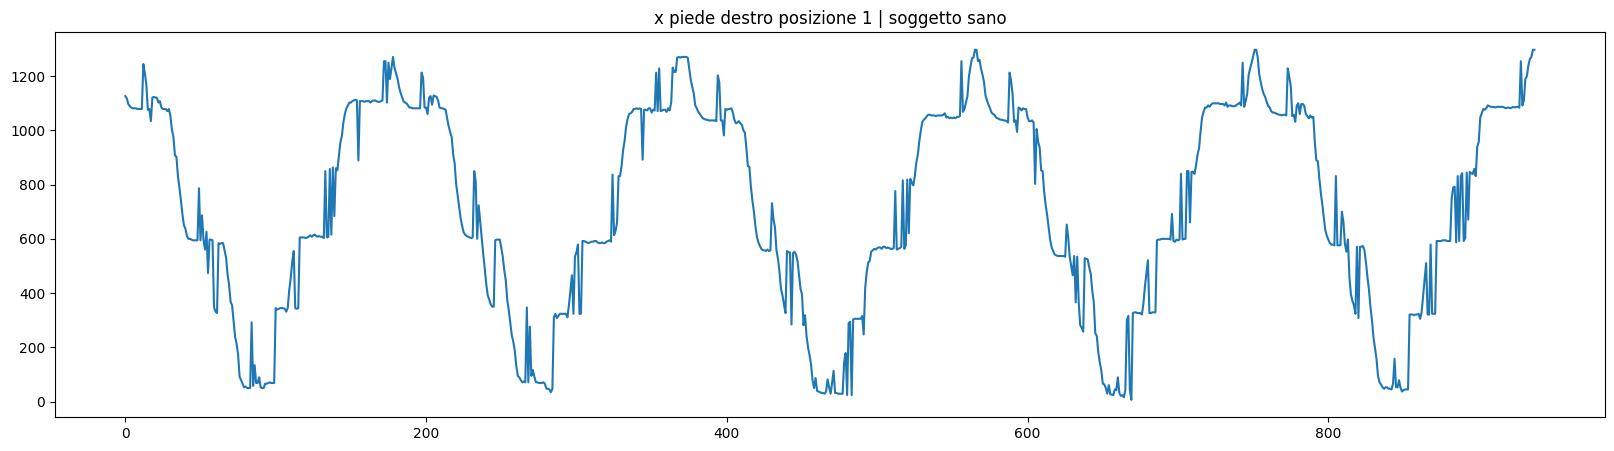
\includegraphics[width=\linewidth,height=4.7cm]{piede_dx_sano_no_filt.png}
    \caption{Piede destro posizione $1$ di un soggetto sano prima dell'applicazione del filtro.}
    \label{fig:piede_dx_1_sano_no_filt}
\end{figure}

\begin{figure}[H]
    \centering
    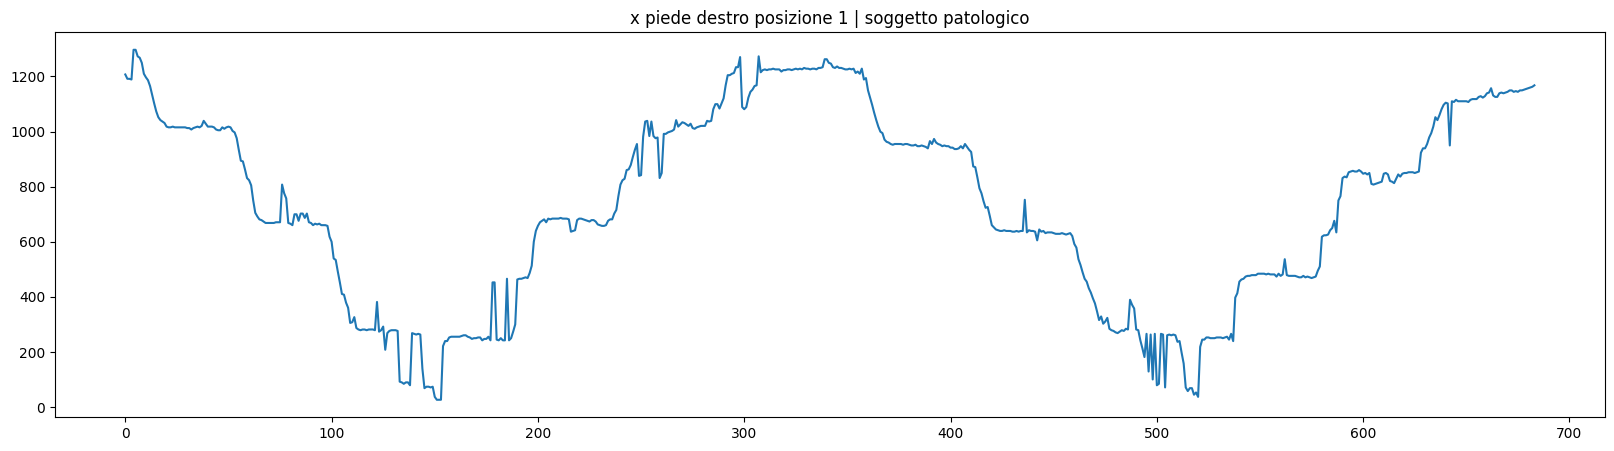
\includegraphics[width=\linewidth,height=4.7cm]{piede_dx_pat_no_filt.png}
    \caption{Piede destro posizione $1$ di un soggetto patologico prima dell'applicazione del filtro.}
    \label{fig:piede_dx_1_pat_no_filt}
\end{figure}

Come possiamo notare dai grafici in figura~\ref{fig:piede_dx_1_sano_no_filt} 
e~\ref{fig:piede_dx_1_pat_no_filt} le serie non sono filtrate e contengono molto rumore.

\begin{figure}[H]
    \centering
    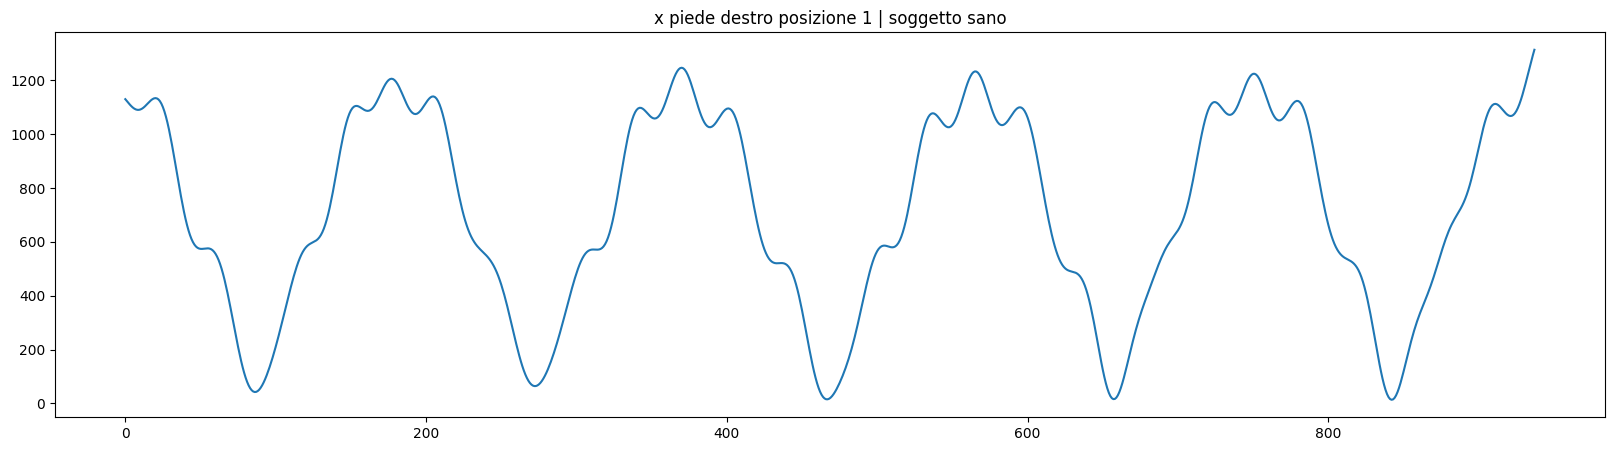
\includegraphics[width=\linewidth,height=4.7cm]{piede_dx_sano_filt.png}
    \caption{Piede destro posizione $1$ di un soggetto sano dopo l'applicazione del filtro.}
    \label{fig:piede_dx_1_sano_filt}
\end{figure}

\begin{figure}[H]
    \centering
    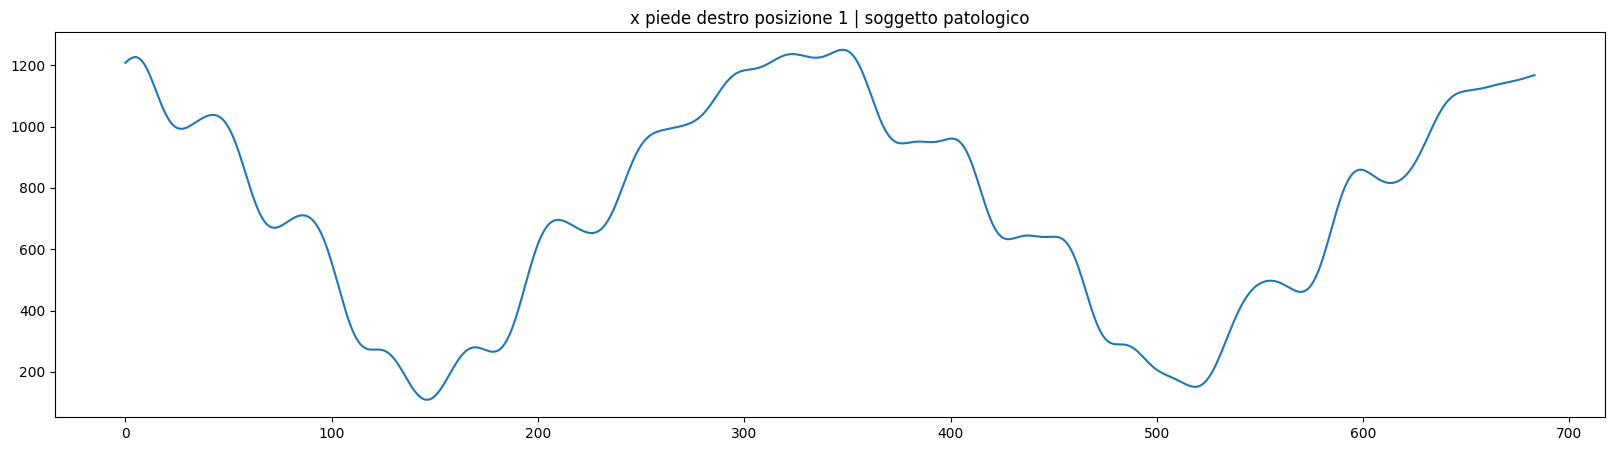
\includegraphics[width=\linewidth,height=4.7cm]{piede_dx_pat_filt.png}
    \caption{Piede destro posizione $1$ di un soggetto patologico dopo l'applicazione del filtro.}
    \label{fig:piede_dx_1_pat_filt}
\end{figure}

l'effetto sinusoidale del grafico rappresenta l'andamento del passo di un soggetto, 
nello specifico se consideriamo il coefficiente angolare delle rette tangenti ai punti del 
grafico, quindi la sua derivata prima, e consideriamo come inizio del passo il 
primo punto in cui la derivata è uguale a $0$ la fine di un passo sarà il punto successivo 
in cui la sua derivata prima è uguale a $0$. 


Dai grafici in figura~\ref{fig:piede_dx_1_sano_filt} 
e~\ref{fig:piede_dx_1_pat_filt} possiamo notare come il filtro ha rimosso il rumore 
presente dalle serie e come l'effetto sinusoidale rimasto rappresenta l'andamento del passo di un soggetto.
nello specifico se consideriamo il coefficiente angolare delle rette tangenti ai punti del 
grafico, quindi la sua derivata prima, e consideriamo come inizio del passo il 
primo punto in cui la derivata è uguale a $0$ la fine di un passo sarà il successivo punto 
in cui la sua derivata prima è uguale a $0$. 

Detto ciò un'ulteriore osservazione possibile sui grafici in figura~\ref{fig:piede_dx_1_sano_filt} 
e~\ref{fig:piede_dx_1_pat_filt} è che si può notare la presenza della periodicità
relativa ad un'andata e ritorno del soggetto,
essendo che sicuramente avviene più lentamente della periodicità di uno stride, essa
risiede nelle frequenze ``molto basse''. 
Per cercare di isolare maggiornmente la caratteristica del passo
si è deciso di eliminare questa periodicità
andando a filtrare con un filtro passa alte le frequenze ``bassissime'' o almeno
abbastanza basse da rimuovere solamente quella periodicità senza 
incidere sulle componenti che caratterizzano lo stride di un soggetto. 
Dopo qualche tentativo
è stato deciso di utilizzare un filtro passa alte con frequenza di taglio $0.5\mathsf{Hz}$
(periodicità che si ripetono ogni $2\mathsf{secondi}$ e superiori) con un ordine di filtro di $10$.

Vediamo ora i grafici delle due serie rappresentate in figura~\ref{fig:piede_dx_1_sano_filt} 
e~\ref{fig:piede_dx_1_pat_filt} a confronto prima e dopo l'ultima fase di filtraggio.

\begin{figure}[H]
    \centering
    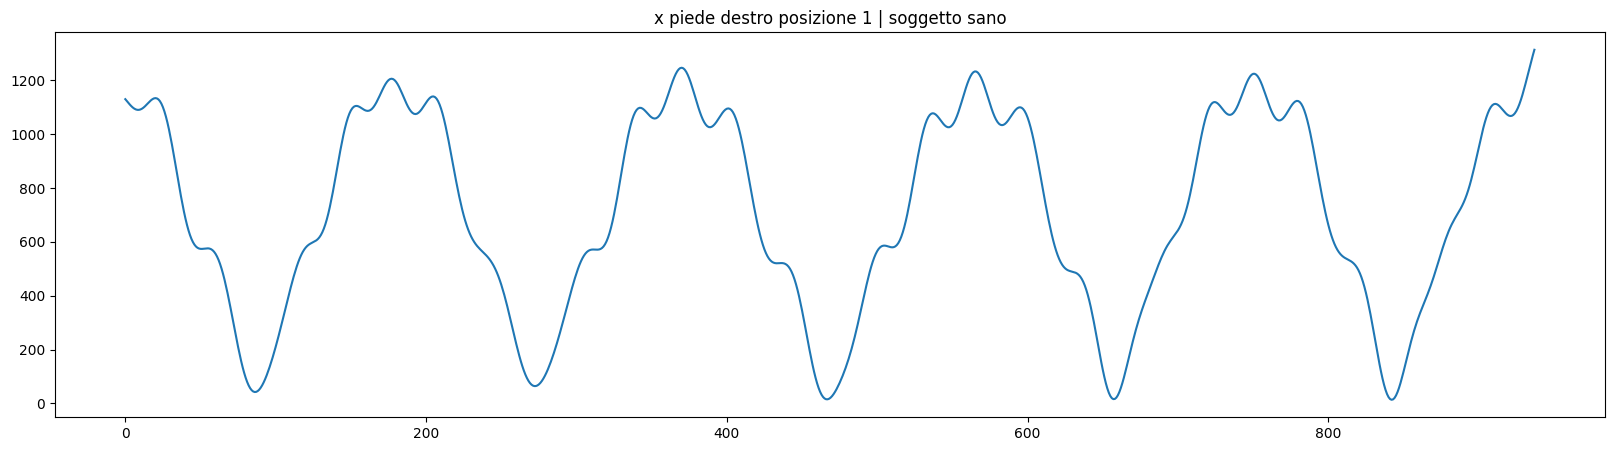
\includegraphics[width=\linewidth,height=4.7cm]{piede_dx_sano_filt.png}
    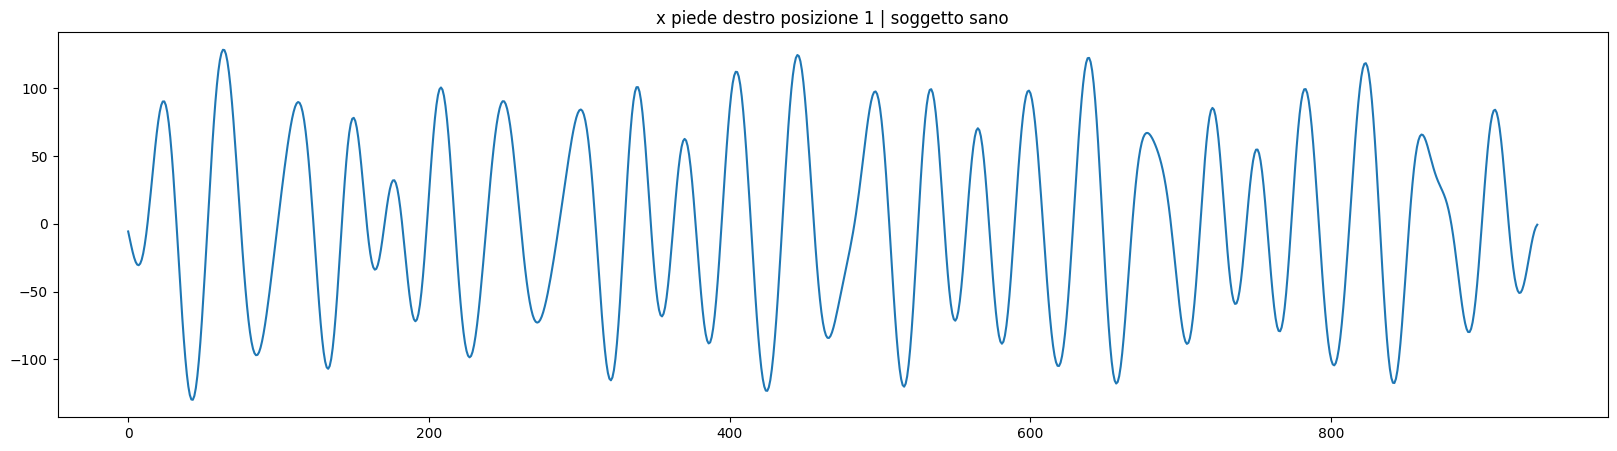
\includegraphics[width=\linewidth,height=4.7cm]{piede_dx_sano_filt2.png}
    \caption{Piede destro posizione $1$ di un soggetto sano prima e dopo l'applicazione dell'ultima fase di filtraggio.}
    \label{fig:piede_dx_1_sano_filt2}
\end{figure}
\begin{figure}[H]
    \centering
    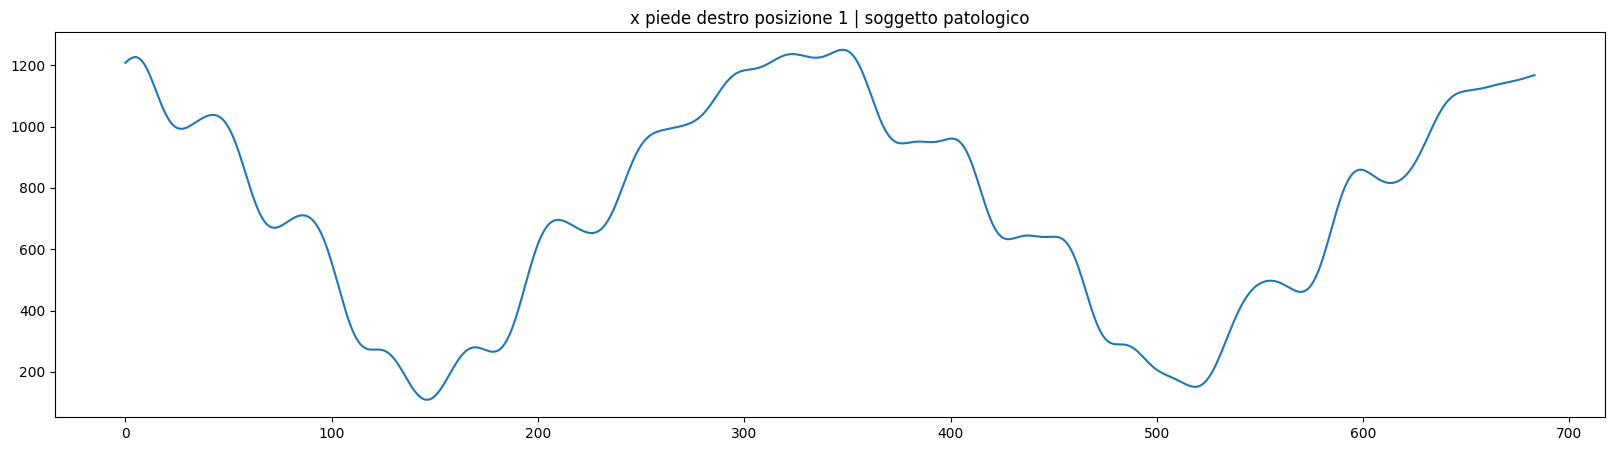
\includegraphics[width=\linewidth,height=4.7cm]{piede_dx_pat_filt.png}
    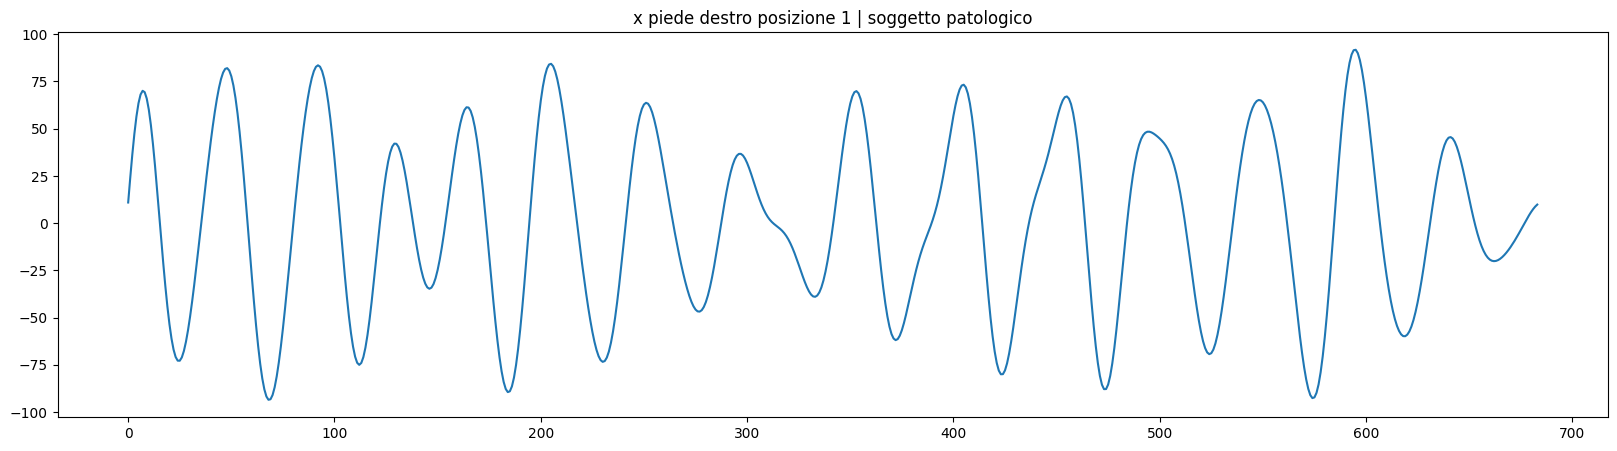
\includegraphics[width=\linewidth,height=4.7cm]{piede_dx_pat_filt2.png}
    \caption{Piede destro posizione $1$ di un soggetto patologico prima e dopo l'applicazione dell'ultima fase di filtraggio.}
    \label{fig:piede_dx_1_pat_filt2}
\end{figure}

Come possiamo notare dai grafici in figura~\ref*{fig:piede_dx_1_sano_filt2} 
e~\ref*{fig:piede_dx_1_pat_filt2} la componente periodica di andata e ritorno 
è stata eliminata 
e consideriamo il secondo grafico di ogni figura possiamo notare come i massimi locali 
delle componenti sinusoidali rappresentino l'inizio di ogni passo del soggetto,
quindi i frame che intercorrono tra un punto di masssimo locale e quello successivo rappresentano
uno stride di un soggetto.
    \section{Analisi del problema e Soluzioni}
In questa sezione verrà descritto il problema affrontato, le soluzioni scelte ed i rispettivi
risultati ottenuti.

\paragraph{Problema affrontato}
Il problema affrontato chiedeva di trovare pattern, anomalie e/o inferire sui dati forniti, 
per ottenere, come risultato, informazioni su di essi mediante l'utilizzo di tecniche 
dell'analisi di serie temporali, e quindi successivamente capire se quest'ultime possano essere 
utlizzate come tencniche ausiliarie per l'analisi a problemi di questa tipologia.

Per riuscire risolvere il problema posto e per questioni di tempo, il problema è stato 
ridotto all'analisi dei soli giunti del piede, più in particolare,
il tirocinio si è basato sulla ricerca di uno o più metodi utili a trovare la durata del passo
(stride) di un soggetto con una successiva analisi dei risultati.



\paragraph{Risultati attesi}
\begin{sloppypar}
Come risultato atteso è stata presa in considerazione l'eventualità della non riuscita dell'obbiettivo finale,
quindi l'impossibilità di trovare, tramite le tecniche dell'analisi di serie temporali, una possibile soluzione
al problema.
\end{sloppypar}

In caso positivo, quindi di una possibile soluzione al problema posto, i risultati attesi potrebbero essere:
\begin{itemize}
    \setlength\itemsep{-0.5em}
    \item Capacità da parte del metodo sviluppato di rilevare la durata del passo.
    \item Capacità da parte del metodo sviluppato di rilevare incorrettamente la durata del passo.
    \item Impossibilità da parte del metodo sviluppato di rilevare un passo.
\end{itemize}


\subsection{Prima soluzione}
In questa sezione verrà mostrata la prima soluzione al problema posto, nello specifico verrà
spiegata in breve l'idea generale, l'implementazione di alcuni dei metodi utilizzati, l'analisi dei
risultati, l'analisi della complessità ed infine le conclusioni.


\subsubsection{Idea generale}
L'idea generale, fulcro di questa soluzione, ruota intorno all'analisi della funzione di autocorrelazione.
Quest'ultima viene utilizzata per riconoscere pattern o una sorta di correlazione tra i dati non
visibile direttamente.

\subsubsection{Implementazione}
Come primo step implementativo è stato necessario scrivere una funzione che rendesse ogni serie stazionaria 
mediante l'ausilio del test di Dickey-Fuller ed il calcolo della prima differenza. Ovviamente
per rendere una serie stazionaria esistono anche altri metodi diversi dalla prima differenza ma 
si è deciso di utilizzarle quest'utlima per la sua semplicità.
\\
\paragraph*{Snippet} (\textit{Prima differenza})
\begin{minted}{python3}
    def compute_first_diff(series: list | np.ndarray):
        """ Calcola la prima differenza
        """
        
        if not isinstance(series, np.ndarray):
            series = np.array(series)

        return series[1:] - series[:len(series)-1]
\end{minted}

\paragraph*{Snippet} (\textit{Metodo per rendere la serie stazionaria})
\begin{minted}{python3}
    def make_stationary(series, max_steps = 30):
        """ Rende la serie stazionaria mediante il calcolo
            della prima differenza
        """
        step = 0   # numero di step
        s_copy = series.copy()  # copia della serie
        
        # fino a quando il test ritornca che la serie
        # non è stazionaria oppure sono stati superati
        # il massimo di step
        while(sts.adfuller(series)[1] > 0.05 
            and step < max_steps):
            
            # calcola la prima differenza
            serie = compute_first_diff(series)
            step += 1

        # se max_step è superato, non si è riusciti
        # a rendere la serie stazionaria
        if step > 30:
            series = s_copy

        return series
\end{minted}

\begin{sloppypar}
Dopo aver reso ogni serie stazionaria è stata applicata la funzione di autocorrelazione ad ognuna di
esse, per capire meglio i risultati di questa operazione prendiamo in cosniderazione alcuni dei 
grafici relativi all'autocorrelazione di serie appartenenti a dataset dei soggetti $6$ ed $12$.
\end{sloppypar}

\begin{figure}[H]
    \centering
    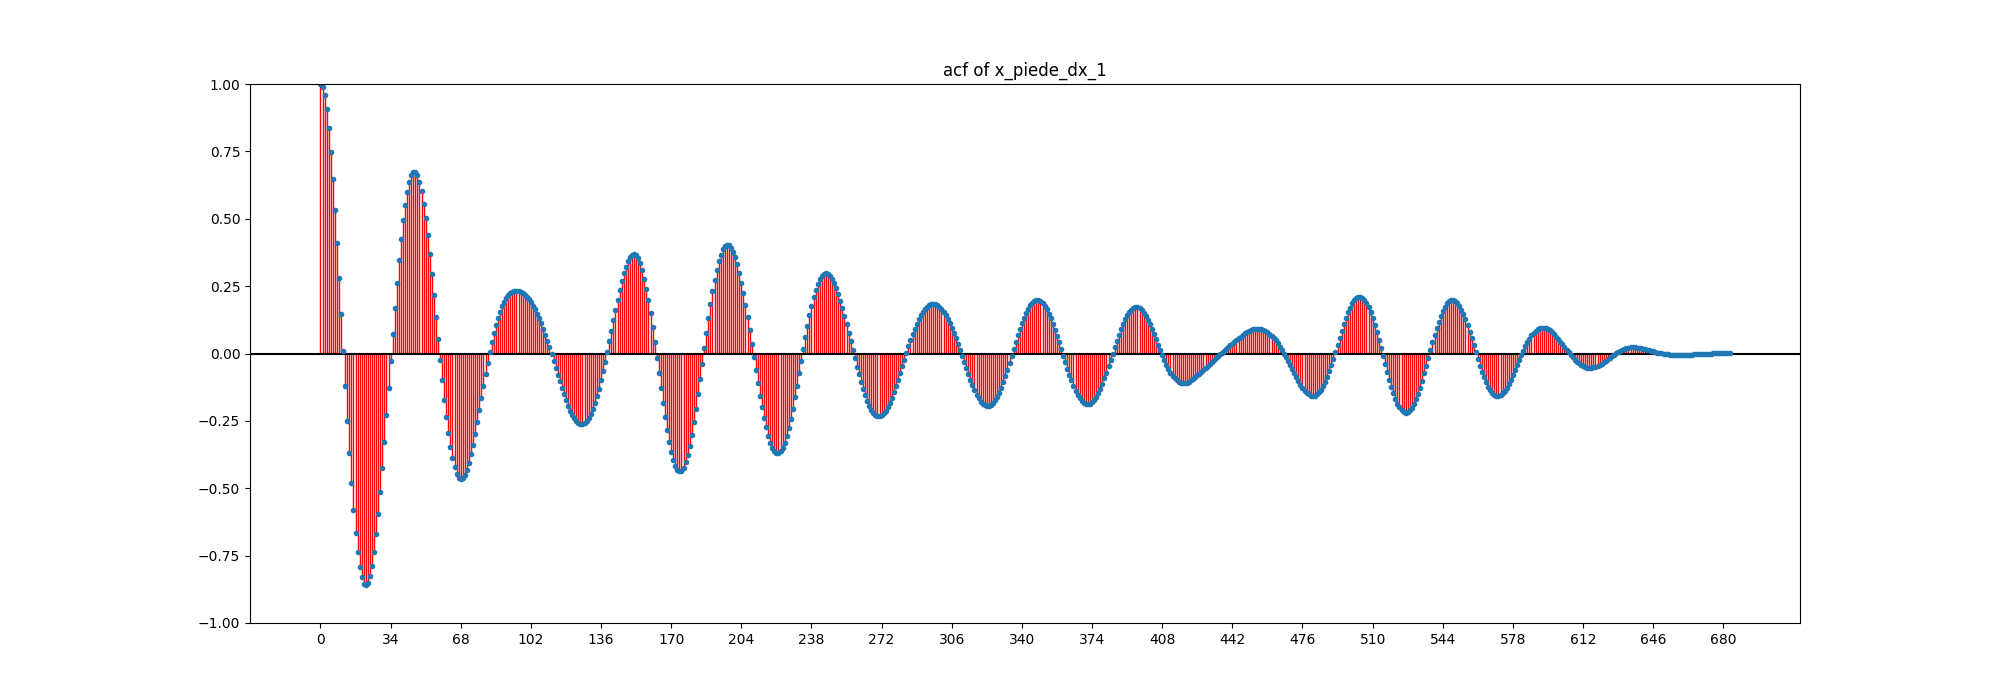
\includegraphics[width=\linewidth,keepaspectratio]{P006_x_piede_dx_1_acf.png}
    \caption{Soggetto $6$ autocorrelazione x piede destro posizione 1.}
    \label{fig:P006_x_piede_dx_1_acf}
\end{figure}

\begin{figure}[H]
    \centering
    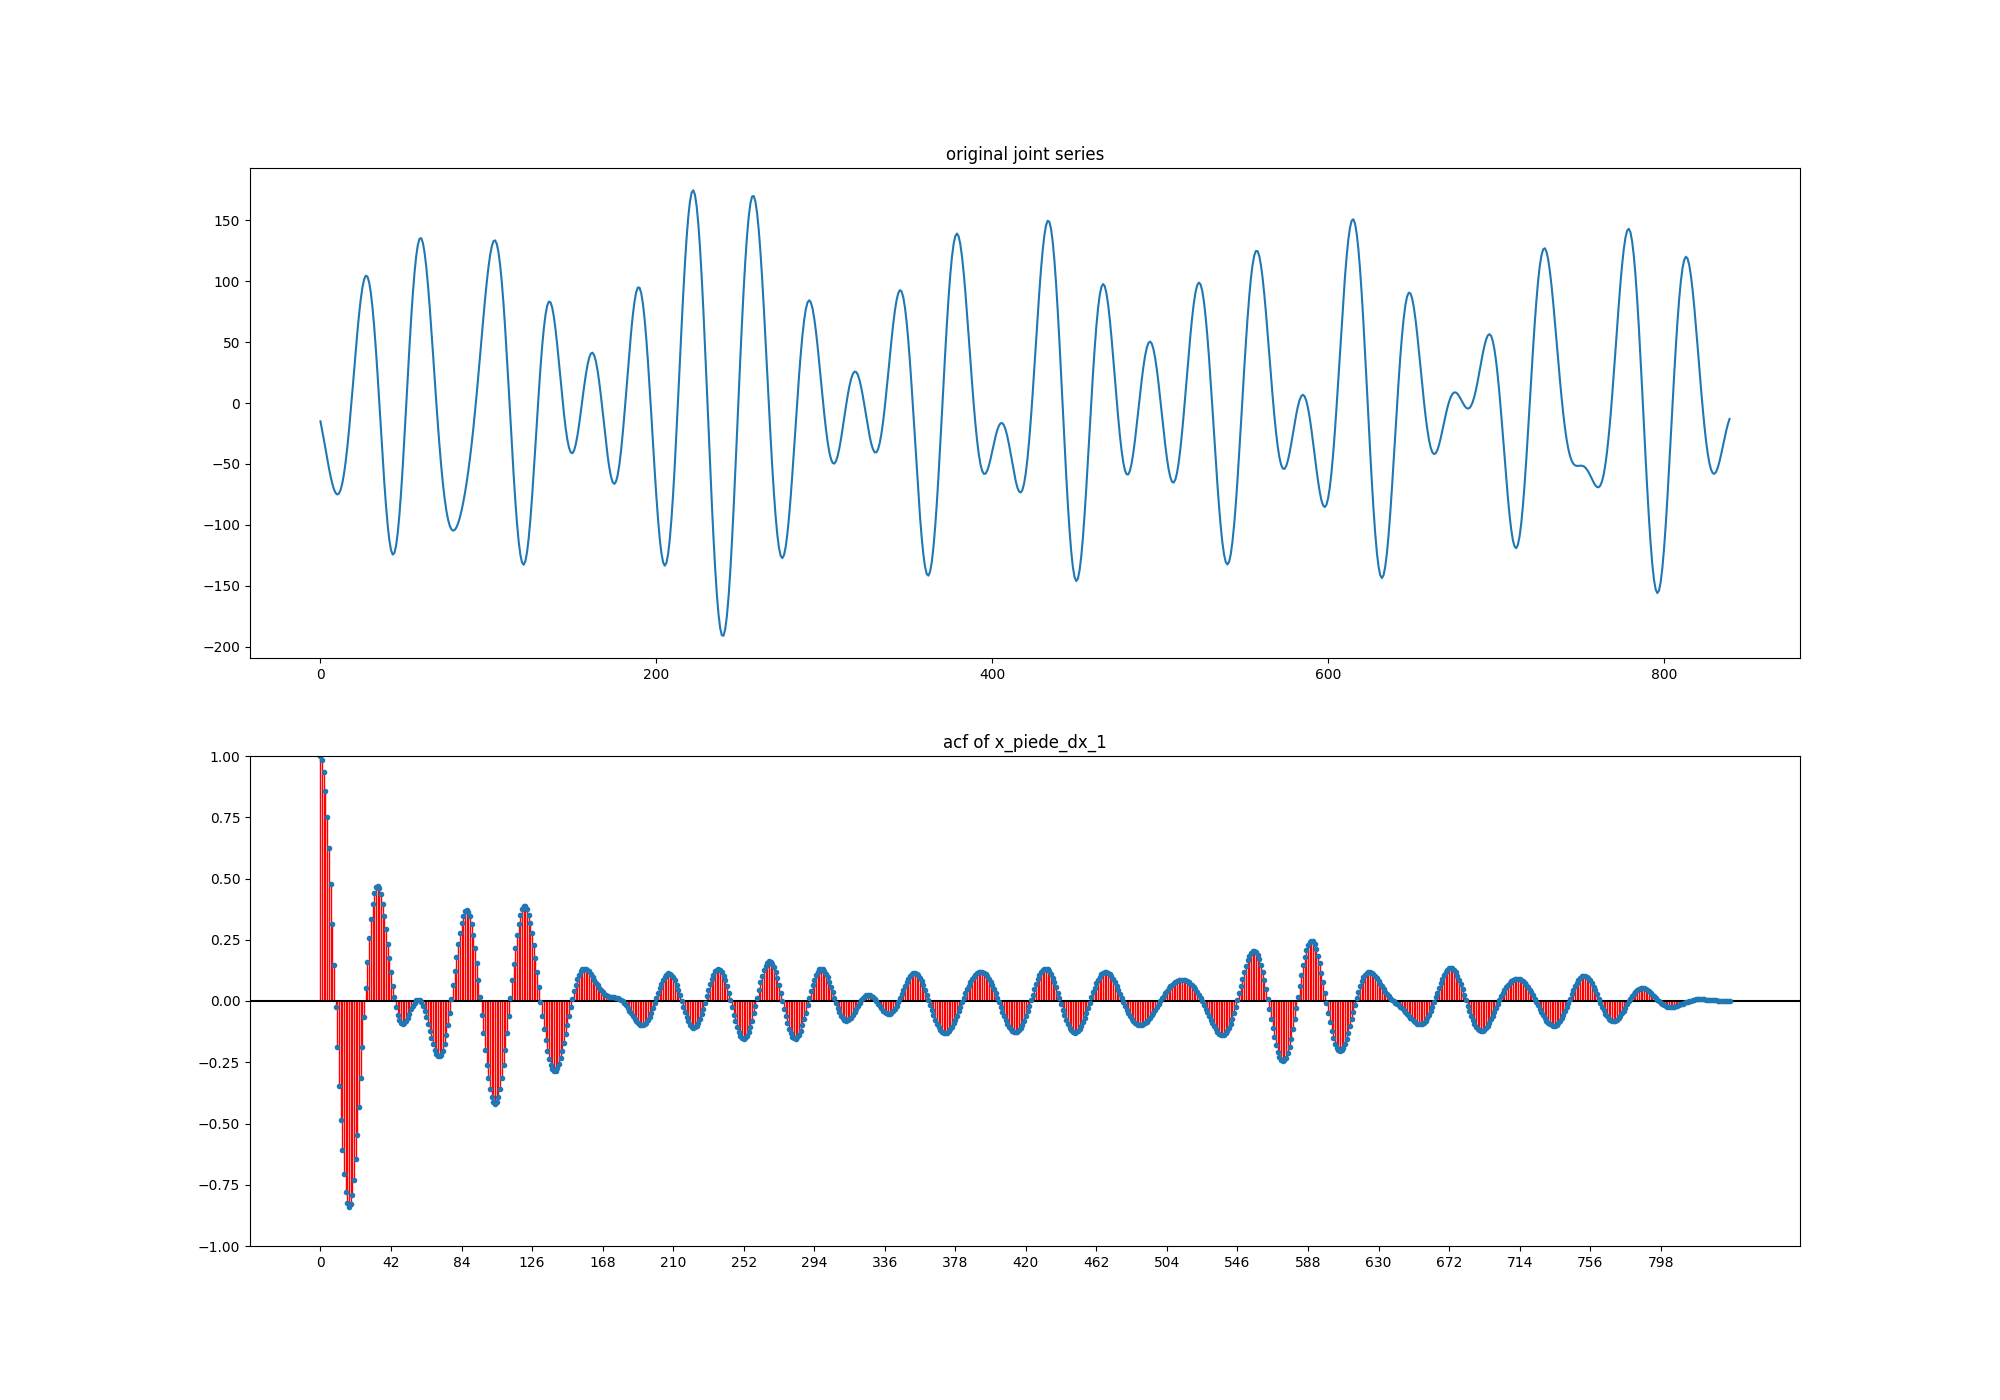
\includegraphics[width=\linewidth,keepaspectratio]{P012_x_piede_dx_1_acf.png}
    \caption{Soggetto $12$ autocorrelazione x piede destro posizione 1.}
    \label{fig:P012_x_piede_dx_1_acf}
\end{figure}

In figura~\ref{fig:P006_x_piede_dx_1_acf} e~\ref{fig:P012_x_piede_dx_1_acf} possiamo vedere
la serie originale in comparazione con il proprio grafico di autocorrelazione. Per entrambi
i grafici troviamo i periodi/frame sull'asse delle ascisse mentre sull'asse delle ordinate 
troviamo l'ampiezza delle sinusoidi, per il grafico rappresentante i dati, ed il livello 
di correlazione, per il grafico dell'autocorrelazione (quanto la serie dei dati è correlata
con una sua versione spostata di $x$ frame/lag).

Nella maggior parte dei casi possiamo inoltre notare come i punti di massimo locale del grafico
dell'autocorrelazione corrispondono all'inizio di un passo, più in precisione corrispondono 
alla ripetizione/pattern relativo ad un passo.

Per capire meglio come interpretare il grafico dell'autocorrelazione vediamo come essa si comporta
con una normale sinusoide (coseno e seno).

\begin{figure}[H]
    \centering
    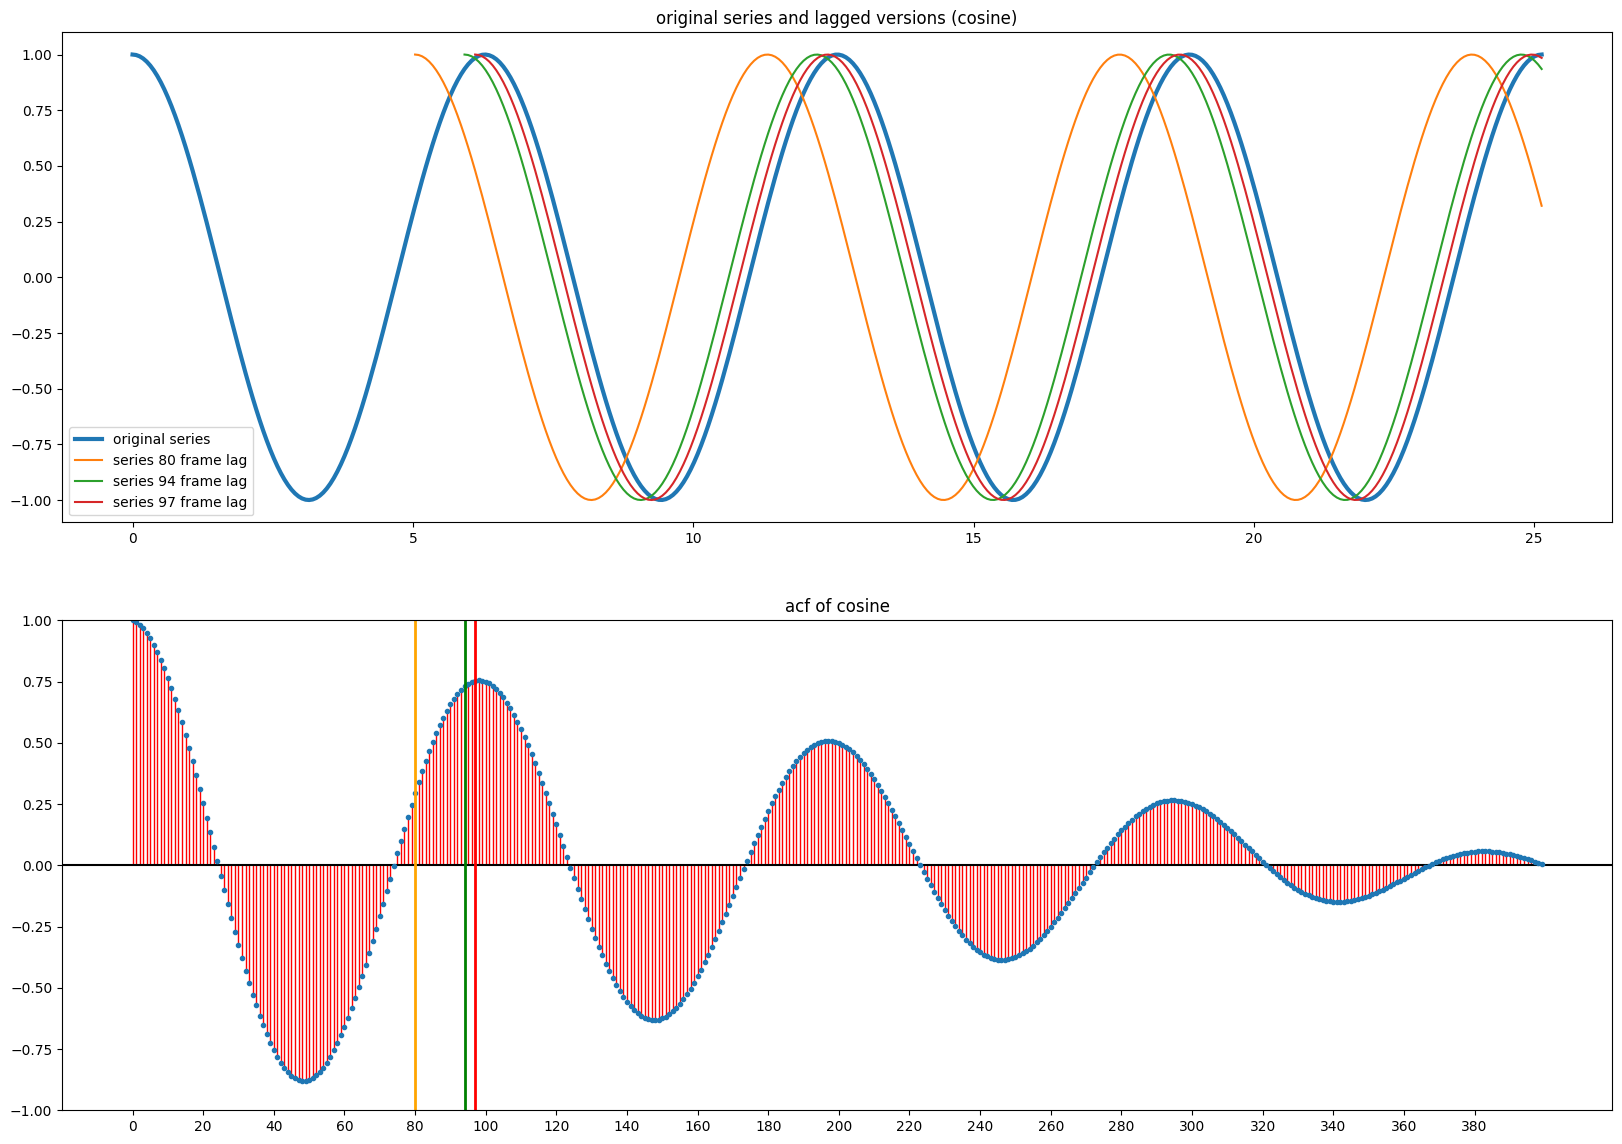
\includegraphics[width=\linewidth,keepaspectratio]{acf_cosine.png}
    \caption{Grafico di un coseno con sue versioni shiftate ed autocorrelazione.}
    \label{fig:acf_cosine}
\end{figure}
\begin{figure}[H]
    \centering
    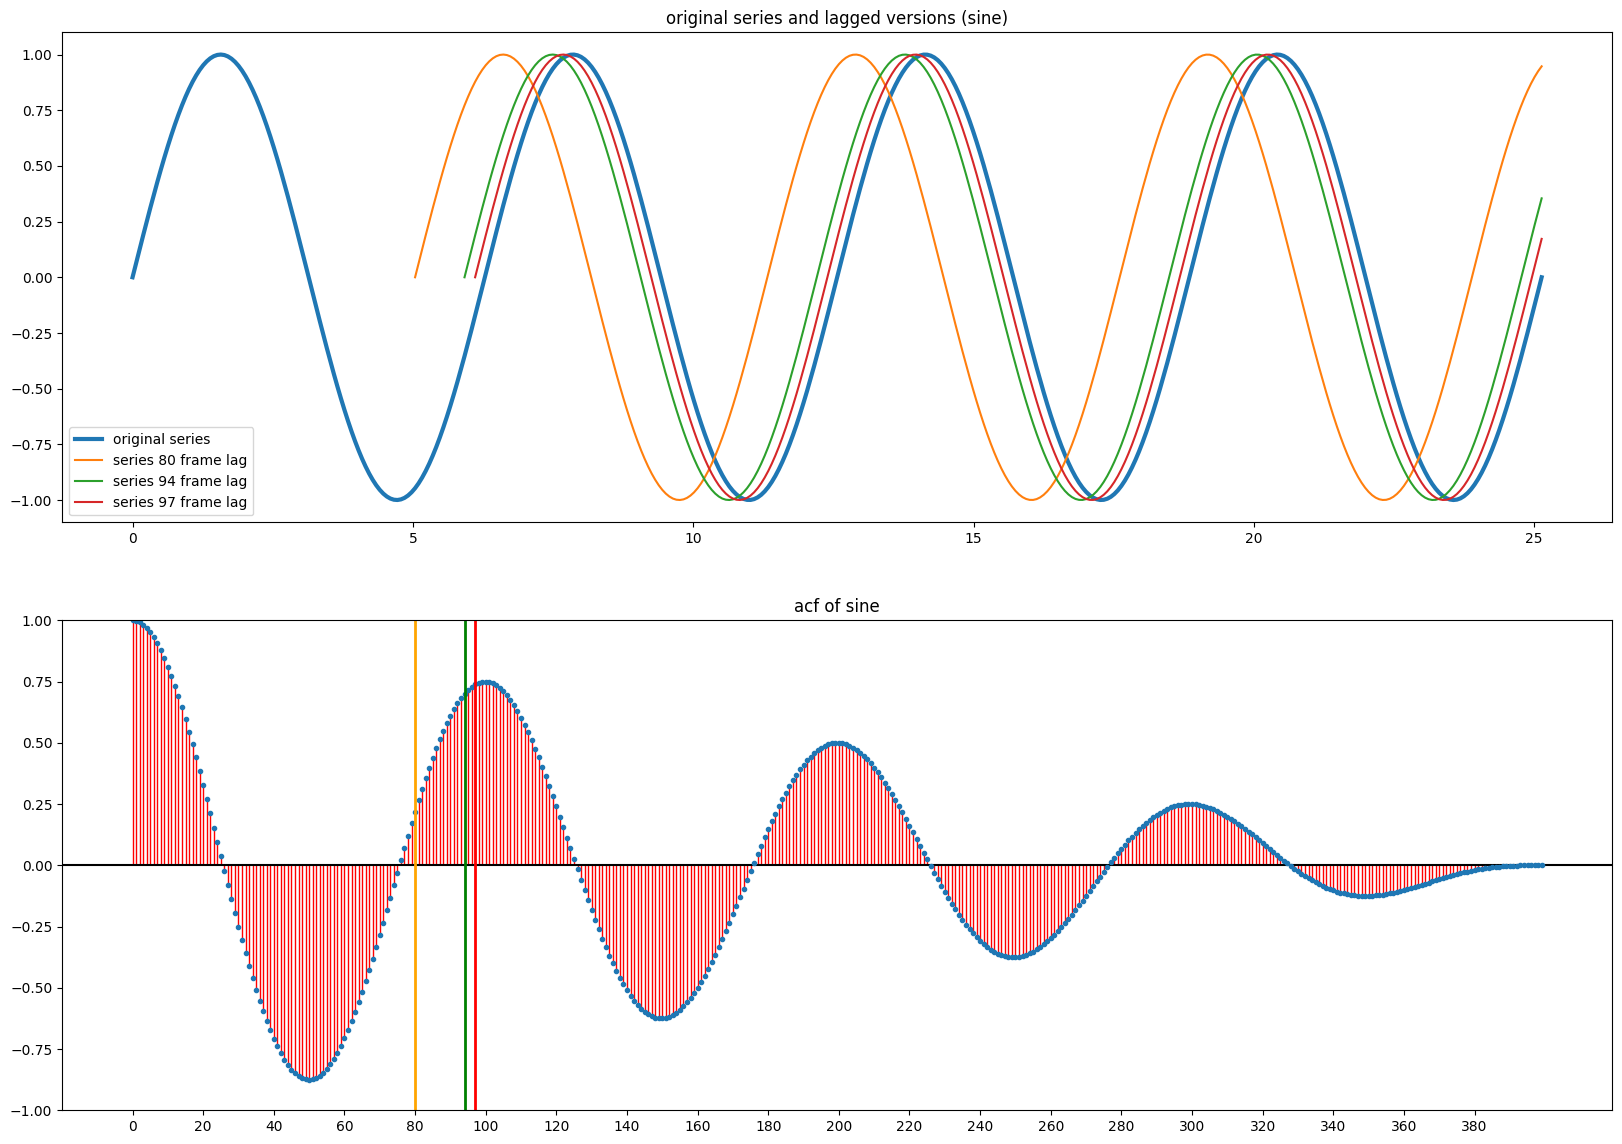
\includegraphics[width=\linewidth,keepaspectratio]{acf_sine.png}
    \caption{Grafico di un seno con sue versioni shiftate ed autocorrelazione.}
    \label{fig:acf_sine}
\end{figure}

Come possiamo vedere dai grafici in figura~\ref{fig:acf_cosine} e~\ref{fig:acf_sine} 
possiamo pensiamo al passo di una persona come un seno oppre ad un coseno. L'idea di utilizzare la
funzione di autocorrelazione nasce dal fatto che quando iniziamo a shiftare la serie
ed iniziamo a sovrapporre i passi, cioè quando le sinusoidi inizieranno ad allinearsi,
la correlazione aumenterà trovando così il pattern di camminata e la durata di uno stride.

\begin{sloppypar}
L'effetto di tendenza a $0$, all'aumentare del numero di frame, nel grafico dell'autocorrelazione,
è dovuto alla funzione di shift, quest'ultima per poter ``spostare'' la serie aggiunge degli $0$
a destra o a sinistra dipendentemente dal verso in cui si vuole eseguire lo shift.
\end{sloppypar}


Per dare un esempio più pratico prendiamo un sottoinseieme della serie relativa al piede 
destro posizione $1$ del soggetto sano $8$.

\begin{figure}[H]
    \centering
    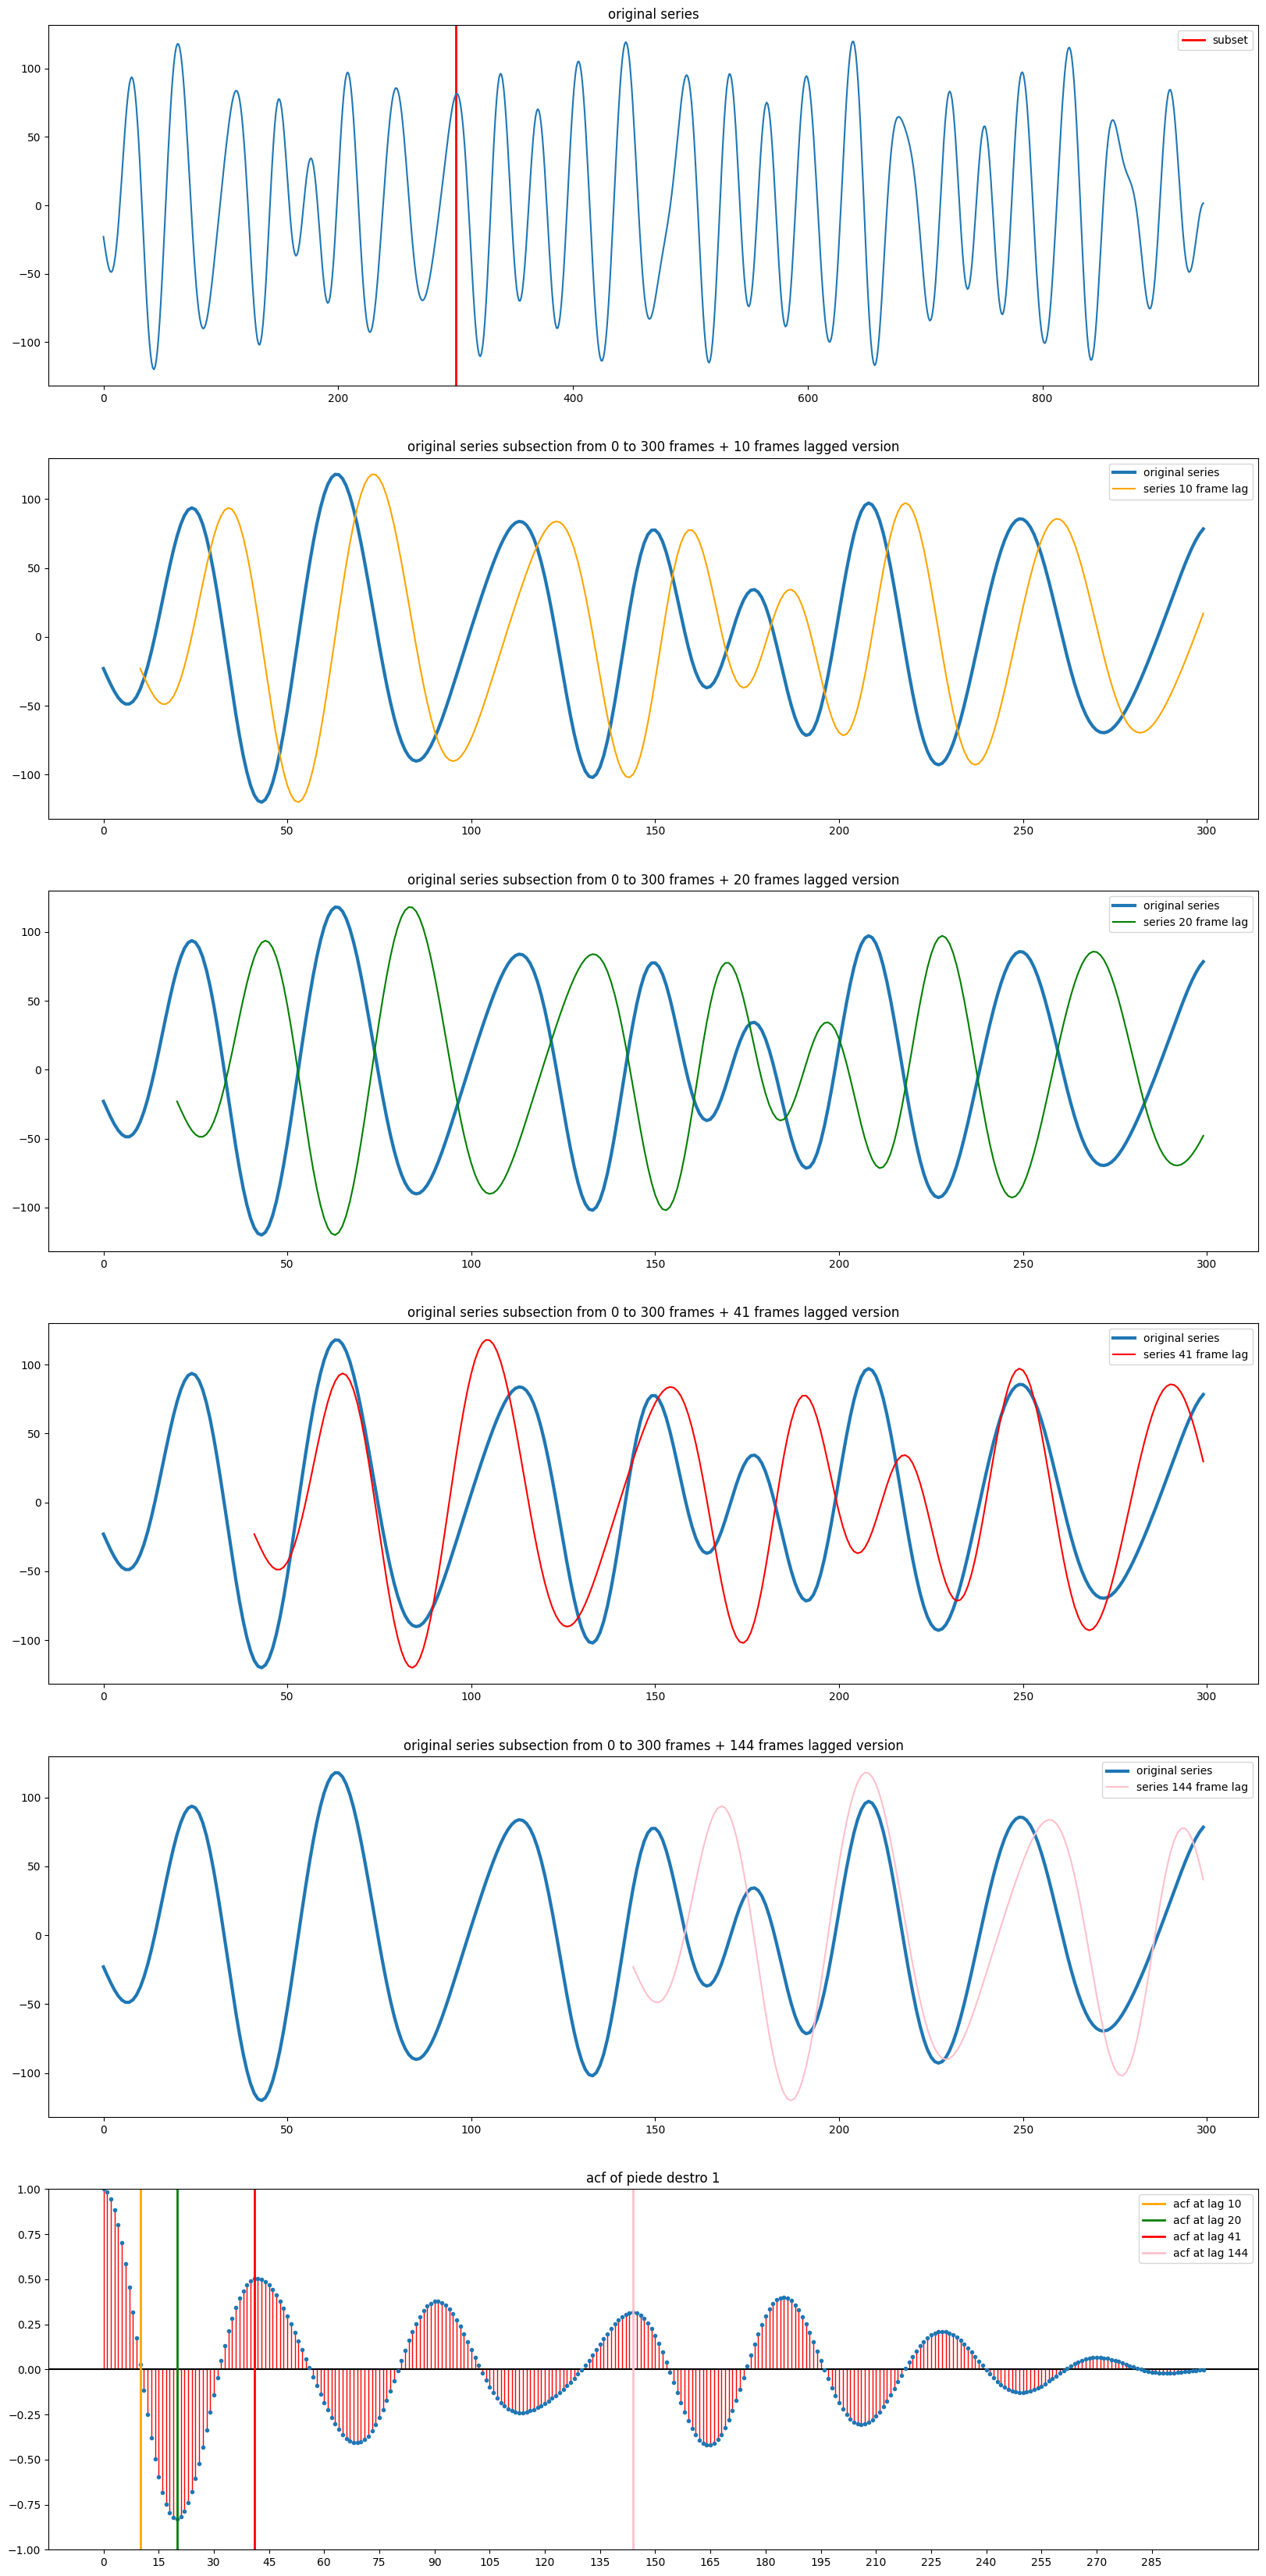
\includegraphics[width=0.8\linewidth,keepaspectratio]{acf_subset_x_piede_dx_008.png}
    \caption{Autocorrelazione con esempi di segnale shiftato.}
    \label{fig:acf_subset_x_piede_dx_008}
\end{figure}
In figura~\ref{fig:acf_subset_x_piede_dx_008} possiamo travere diversi grafici relativi alla
serie del paziente indicato sopra. Spieghiamo ora il loro significato:
\begin{enumerate}
    \item \textbf{Grafico in 1° posizione}: rappresenta la serie originale con una linea rossa (frame $300$)
    che indica il frame finale del sottoinsieme considerato dai grafici sottostanti.
    \item \textbf{Grafico in 2° posizione}:in blu viene rappresento il sottoinsieme preso in considerazione,
    cioè dal frame $0$ al $300$, ed in arancione lo stesso sottoinsieme ma shiftato di $10$ frame/lag.
    \item \textbf{Grafico in 3° posizione}: in blu viene rappresento il sottoinsieme preso in considerazione,
    cioè dal frame $0$ al $300$, ed in verde lo stesso sottoinsieme ma shiftato di $20$ frame/lag.
    \item \textbf{Grafico in 4° posizione}: in blu viene rappresento il sottoinsieme preso in considerazione,
    cioè dal frame $0$ al $300$, ed in rosso lo stesso sottoinsieme ma shiftato di $41$ frame/lag.
    \item \textbf{Grafico in 5° posizione}: in blu viene rappresento il sottoinsieme preso in considerazione,
    cioè dal frame $0$ al $300$, ed in rosa lo stesso sottoinsieme ma shiftato di $144$ frame/lag.
    \item \textbf{Grafico in 6° posizione}: la funzione di autocorrelazione calcolata su tutti i 
    lag possibili con linee di colore arancione, verde, rosso e rosa in prossimità dei valori 
    relativi alla correlazione tra la serie originale e la serie shiftata di $10$, $20$,
    $41$ e $144$ lag (in sostanza sono i valori delle correlazioni relative ai grafici $2$, $3$, $4$ e $5$).
\end{enumerate}

Possiamo notare che il primo valore della funzione di autocorrelazione, cioè il valore della correlazione
tra la seire originale e se stessa, è uguale ad $1$, di logica la massima correlazione possibile si può
avere quando la serie è perfettamente allineata con se stessa.

La correlazione tra la serie originale e la sua versione shiftata di $10$ lag invece ha valore
quasi uguale a $0$, questo perchè se si guarda il grafico numero $2$ in figura, la serie 
original e la sua versione shiftata in colore arancione si ``annullano'' avendo così correlazione
nulla. In altre parole quando la correlazione è vicina a $0$ la serie con la sua versione shiftata
sono ``molto'' diverse.

La correlazione tra la serie originale e la sua versione shiftata di $20$ lag ha un'alta correlazione
ma negativa, infatti se guardiamo il grafico numero $3$ possiamo vedere come la serie originale in blu
e la sua versione shiftata in verde sono una ``l'opposto'' dell'altra trovando così un'alta correlazione
ma negativa. Per poter immaginare una correlazione negativa possiamo pensare alla correlazione della serie
originale con una sua versione ribaltata sull'asse delle ascisse (in sostanza se $y$ è la nostra serie consideriamo $-y$),
il valore della correlazione a lag $0$ varrà $-1$.

Infine se consideriamo la correlazione tra la serie originale e la sua versione shiftata di $41$ lag
essa avrà un valore positivo ma ovviamente non $1$, se guardiamo il grafico numero $4$ possiamo notare
come la serie originale in blu e la serie shiftata in rosso tendano ad allinearsi, avendo così
come risultato una correlazione positiva.

Capito ora come poter interpretare la funzione di autocorrelazione relativa ad una serie 
continuiamo con l'implementazione della soluzione proposta.

\begin{sloppypar}
Utilizzando la funzione \texttt{argrelextrema} del modulo \texttt{statsmodels.tsa.stattools}
all'output della funzione di autocorrelazione è stato possibile recuperare gli argomenti (indici della lista) dei massimi locali.
Per esempio se prendiamo in considerazione il grafico~\ref{fig:P006_x_piede_dx_1_acf} gli argomenti
dei massimi locali sono
\end{sloppypar}
\[ [45, 95, 152, 197, 245, 297, 347, 395, 454, 504, 549, 592, 636, 678] \]
dove ogni argomento fa riferimento all'istante di tempo $t$, quindi al frame, in cui uno stride si ripete.

\begin{sloppypar}
Questo ovviamente succede in linea teorica, non sempre è detto che il grafico dell'autocorrelazione
riesca ad ottenere con precisione quest'informazione, soprattutto se i dati non sono filtrati correttamente.
\end{sloppypar}

Continuado con l'implementazione del metodo, calcolando la distanza tra un argomento e l'altro troveremo
la durata di quel determinato passo. Prendendo sempre in considerazione la lista di agromenti sopra
e calcolandone la prima differenza otterremo
\[[50, 57, 45, 48, 52, 50, 48, 59, 50, 45, 43, 44, 42]\]
dove ogni elemento rappresenta la durata di un singolo stride.

Se calcoliamo la media otterremo la durata media di uno stride, che per la lista sopra sarà di 
$48.69\texttt{frame}$ cioè $1.623\texttt{secondi}$.


\paragraph{Snippet} (\textit{Metodo per il calcolo dello stride})
\begin{minted}{python3}
    def stride(serie: list | np.ndarray):
        """ Calcola la durata di uno stride
            assumendo che la serie sia stazionaria    
        """

        # redi la serie un array numpy
        if not isinstance(serie, np.ndarray):
            serie = np.array(serie)
        
        # funzione di autocorrelazione
        acf = funzione_autocorrelazione(serie)

        # prende gli argomenti massimi locali della acf
        arg_max_locali = argrelextrema(acf, np.greater)[0]

        # differenza tra gli argomenti massimi locali
        arg_max_locali_diff = compute_first_diff(arg_max_locali)

        # calcola durata media di uno stride
        media_stride = arg_max_locali_diff.mean()

        if not isinstance(serie, np.ndarray):
            arg_max_locali_diff = arg_max_locali_diff.tolist()

        return arg_max_locali_diff, media_stride

\end{minted}


Questa serie di metodi è stata successivamente applicata ad ogni dataset ottenendo così la durata
media di uno stride per ogni posizione del piede destro e sinistro. Per fare ciò è stato creato
un ``mini'' programma che esegue automaticamente queste istruzioni ad ogni serie.

\subsubsection{Analisi di complessità}
\begin{sloppypar}
Assumendo che la serie fornita sia già stazionaria la complessità di questo algoritmo 
deriva pricipalmente dalla complessità della funzione \texttt{funzione\_autocorrelazione} e dalla complessità
della funzione \texttt{singola\_autocorrelazione} utilizzata dalla funzione di autocorrelazione.

Se consideriamo $n$ come la lunghezza della serie, 
la funzione \texttt{autocorrelazione\_singola} ha complessità temporale e spaziale $O(n)$ quindi
la funzione \texttt{funzione\_autocorrelazione} avrà complessità temporale $O(n^2)$ e complessità
spaziale $O(n)$.
\end{sloppypar}


\subsubsection{Analisi dei risultati e Conclusioni}
Per seplicità, i risultati verranno analizzati considerano un passo completo, cioè la somma degli stride
del piede destro e sinistro. Per fare chiarezza mostriamo un'immagine.
\begin{figure}[H]
    \centering
    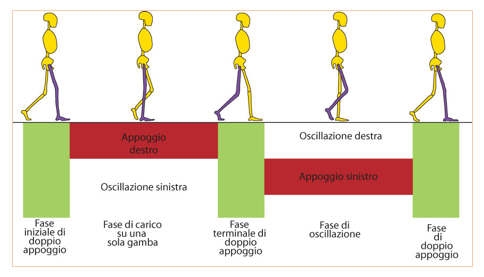
\includegraphics[width=0.8\linewidth,keepaspectratio]{passo_completo.png}
    \caption{Camminata di un soggetto~\cite{cf:passo_completo}.}
    \label{fig:passo_completo}
\end{figure}
Considerando la figura~\ref*{fig:passo_completo} stiamo valutando il periodo (durata) che parte dalla prima striscia
verde fino all'ultima striscia verde, quindi dall'inizio di una fase iniziale di doppio appoggio fino all'inzio
di un'altra fase iniziale di doppio appoggio.

\begin{sloppypar}
Detto ciò, compariamo ora la durata media dei passi completi dei soggetti sani e patologici. 

Si è trovato che la durata media di un passo completo con camminata normale è di rispettivamente $68,84 \ \texttt{frame}$
($2,294 \ \texttt{secondi}$) per i soggetti sani e di 
$81,71 \ \texttt{frame}$ ($2,723 \ \texttt{secondi}$) per i soggetti patologici.
I soggetti patologici, con camminata normale, hanno quindi una durata di passo completo maggiore del 
$19,84\%$ rispetto alla durata di un passo completo, con camminata normale, dei soggetti sani.
\end{sloppypar}

Applicando lo stesso ragionamento alle camminata tacco-punta e punta si è riscontrato che 
i soggetti patologici, con camminata tacco-punta, hanno una durata di passo completo maggiore del 
$8.28\%$ rispetto alla durata di un passo completo, con camminata tacco-punta, dei soggetti sani, 
mentre nella camminata punta si è riscontrata una durata maggiore del $43,04\%$.

I risultati ottenuti analizzando i dati delle camminate tacco-punta e punta non possono ritenersi affidabili
in quanto le percentuali e le medie sono state calcolate con troppe poche osservazioni.


\paragraph*{Premessa sui risultati}
I risultati sopra ottenuti non sono da prendere come riferimento in quanto essi sono ottenuti
mediante l'ausilio di un metodo non totalmente sicuro. Il metodo utilizzato è sperimentale e tantomeno 
fine allo scopo del tirocinio quindi potrebbe giungere a risultati non corretti 
poiché la funzione di autocorrelazione potrebbe rilevare pattern e correlazioni diverse da quelle
aspettate ed anche perché questa tecnica è stata applicata a serie filtrate in un certo modo.

\paragraph*{Problemi non totalmente risolti o ancora incogniti}
Una incognita rimasta aperta dopo l'analisi dei grafici dell'autocorrelazione e delle serie originali
è l'effetiva importanza in questa soluzione di rendere le serie stazionarie. 
La funzione di test Dickey-Fuller per l'analisi della stazionarietà fornita dal 
pacchetto \texttt{statsmodels} ha la possibilità
di capire automaticamente il numero di lag su cui eseguire il test e, per come è stato implementata
la soluzione, l'algoritmo rileva un numero di lag non sufficiente per ottenere un risultato 
di test veritiero.

Considerato il fatto che la funzione della soluzione che rende le serie stazionarie non 
rileva propriamente quando una serie è stazionaria, e quindi tutte le analisi successive
sono state eseguite su serie non propriamente stazionarie, i risultati ottenuti non sono
si discostano molto dalla realtà. Questo potrebbe essere dovuto a come sono stati
filtrati i dati in partenza, e quindi, per questa determinata applicazione, non è stato necessario 
avere delle serie propriamente stazionarie.

In breve con lo sviluppo di questa soluzione e l'interpretazione dei risultati ottenuti
non si è riuscita a cogliere l'importanza di avere una serie stazionaria non trovando
molta differenza tra una serie stazionaria ed una non stazionaria (sempre rimanendo nei
limiti di quest'applicazione).

\subsection{Seconda Soluzione}
In questa sezione verrà mostrata la seconda soluzione al problema posto, nello
specifico verrà spiegata in breve l’idea generale, l’implementazione di alcune parti relative all'algoritmo, 
l’analisi dei risultati, l’analisi della complessità ed infine
le conclusioni.

\subsubsection{Idea generale}
In questa soluzione al problema si è pensato di considerare la scoposizione delle serie nelle 
loro componenti quali trend, stagionalità e residui. Nello specifico l'idea è nata
pensado che possiamo considerare ad un passo (stride) di un soggetto come ad un evento periodico
che si ripete più o meno in ugual maniera nel tempo ad uno specifico periodo. Considerando quindi
la scoposizione nelle tre compnenti di una serie, la stagionaità ad un determinato periodo potrebbe
rappresentare l'informazione che stiamo cercando di ottenere. Questo avviene solamente il linea teorica
in quanto non è detto che il passo di un soggetto avvenga sempre ad intervalli precisi ma l'idea è che
ad un certo periodo la stagionalità raccolga la maggior parte dell'informazione cercata.

Essendo che questo processo si può provare attuare solamente guardando il grafico della stagionalità
si è pensato di automatizzarlo cercando un algoritmo che, data una serie temporare relativa ad un giunto,
esso dia come risultato un periodo
la cui stagionaità raccolga la maggior parte dell'informazione di un passo. Per fare ciò è stato 
necessario comparare due serie, o meglio detto, è stato necessario comparare la serie relativa 
ad un giunto divisa a metà considerando le due metà come serie separate. Successivamente
si è calcolata la stagionalità su più periodi per entrambe le serie. In linea teorica i periodi con
stagionalità simili sarebbero dovute essere i pattern che occorrono in entrambe le serie,
mentre le stagionalità ``diverse'' sarebbero dovute essere pattern che non rientrano 
in entrambe probabilmente dovuto ad altre motivazioni quali, ad esempio, del rumore ancora presente.





\subsubsection{Implementazione}
Per prima cosa è necessario dividere una serie relativa ad un giunto di un soggetto in due e decidere
su quali periodi calcolare la stagionalità.

\begin{sloppypar}
Successivamente per ogni periodo si è calcolata la stagionalità delle due parti
calcolandone la differenza quindi l'errore tra le due stagionalità. Per calcolare la stagionalità
è stata utilizzata la funzione \texttt{seasonal\_decompose} del modulo \texttt{statsmodels.tsa.seasonal}
relativo al pacchetto \texttt{statsmodels}, mentre per il calcolo dell'errore
le due stagionalità sono state convertite nel dominio delle frequenze, utilizzando la trasformata
di Fourier, e calcolata la differenza di ampiezza tra frequenze. L'algoritmo è stato 
creato per poter accettare anche serie divise in più di due parti.
\end{sloppypar}

Vediamo ora come è stata implementata la funzione che esegue il calcolo dell'errore.

\paragraph*{Snippet} (\textit{Calcolo dell'errore tra stagionalità})
\begin{minted}{python3}
    def freq_error(season_1: list, season_2: list):

        # prendi la lunghezza minima 
        min_len = 0
        if len(season_1) < len(season_2):
            min_len = len(season_1)
        else:
            min_len = len(season_2)

        # calcolo della trasformata di 
        # Fourier tra stagionalità
        fft_season_1 = sft.fft(season_1, min_len)
        fft_season_2 = sft.fft(season_2, min_len)

        # calcolo del magnitudo per ogni trasformata
        fft_season_1_m = np.abs(fft_season_1) / len(season_1)
        fft_season_2_m = np.abs(fft_season_2) / len(season_2)

        # differenza tra frequenze
        fft_diff = []
        for idx in range(min_len//2):
            fft_diff.append(fft_season_1_m[idx] - fft_season_2_m[idx])
        
        # calcolo dell'errore quadratico medio
        return np.power(fft_diff, 2).mean() 
\end{minted}


Vediamo ora il metodo principale.
\paragraph*{Snippet} (\textit{Metodo per la soluzione al problema (2)})
\begin{minted}{python3}
    def soluzione_2(seriesList, periods):
        """ 
        seriesList = 
                lista che contiene la serie divisa in due parti
                quindi due liste

        periods = 
                lista di interi, è la lista che
                contiene i periodi su cui calcolare
                la stagionalità
        """
        # per ogni periodo
        errors = []
        for j, period in enumerate(periods):

            # non è possibile calcolare 
            # la stagionalità per il periodo 0
            if period == 0:
                raise Exception('stagionalità non calcolabile \
                    con periodo 0')

            # calcola l'errore le parti della serie
            aux_errors = []
            for idx, series in enumerate(seriesList):

                # stagionalità della prima parte
                season = seasonal_decompose(
                    series, period=period).seasonal

                
                for idx in range(idx+1, len(seriesList)):

                    # stagionalità della seconda parte 
                    # (e altre parti)
                    aux_season = seasonal_decompose(
                        seriesList[idx], period=period).seasonal
                    
                    # calcolo dell'errore tra stagionalità
                    aux_errors.append(
                        freq_error(season, aux_season)
                    )
            

            errors.append(np.mean(aux_errors))

        return np.min(errors), periods[np.argmin(errors)], errors
\end{minted}

Come possiamo vedere dall'implementazione come risultato otteniamo l'errore minimo, il periodo
associato all'errore minimo e la lista contenente, per ogni periodo, l'errore associato.

In una fase successiva è stata creata una funzione che permette di analizzare la lista relativa
agli errori per ogni periodo creando dei grafici che indicano i periodi ``salienti''. 
L'implementazione di quet'ultima non verrà data ma il concetto è che per periodi piccoli l'errore
è sempre il minimo e crescente e, dopo un certo periodo, l'errore inizia ad aumentare drasticamente
per poi diminuire successivamente dopo aver trovato una stagionalià nuovamente simile tra le due serie.
Per capire meglio consideriamo la lista degli errori tra $1$ e $30$, in questo range l'errore è crescente
per ogni periodo, dal periodo $31$ in poi l'errore aumenta drasticamente fino al periodo $80$ per poi diminuire
nuovamente ed ad un certo punto riaumentare. Questo è dovuto appunto al fatto che quando le stagionalità non si
``assomigliano'' l'errore sarà alto mentre per stagionalità simili l'errore è minimo o comunque molto basso.

\subsubsection{Analisi di complessità}
Consideriamo come $m$ il numero di sottoinsiemi, di ugual lunghezza, creati a partire da una serie 
(negli esempi sopra abbiamo sempre considerato di dividere la serie in due parti),
$n$ la lunghezza di un sottoinsieme, $S$ la complessità della 
funzione \texttt{seasonal\_decompose} e tenuto conto che il periodo massimo su cui è possibile
calcolare quest'ultima è di $(m/2)$, la complessità temporale della seconda soluzione è 
$O( (n/2)m\log{(m)}Sn\log{(n)} )$ mentre la complessità spaziale sarà $O( n+2n+(n/2) )$ quindi $O(n)$.


\subsubsection{Analisi dei risultati e Conclusioni}
Analizziamo ora qualche grafico cercando di capire meglio come rappresentare i risultati del metodo
spiegato nella sezione precedente.
\begin{figure}[H]
    \centering
    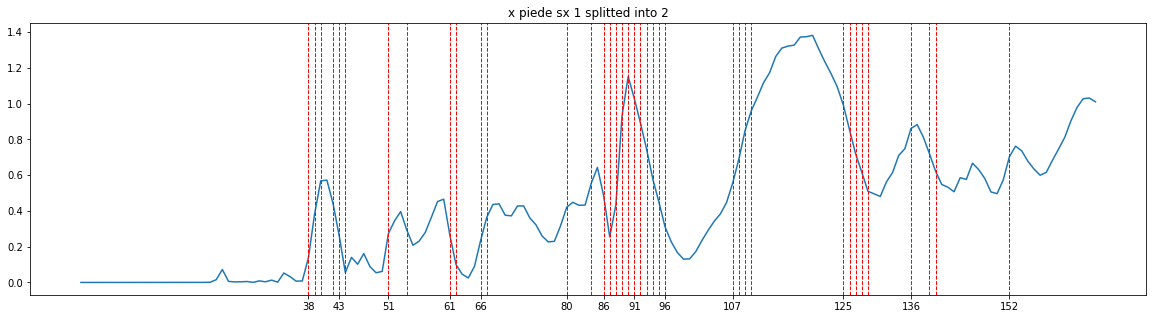
\includegraphics[width=0.8\linewidth,keepaspectratio]{x_piede_sx_1_006.png}
    \caption{Grafico degli errori per ogni periodo relativo al piede sinitro posizione 1 del soggetto patologico $6$.}
    \label{fig:x_piede_sx_1_006_m2}
\end{figure}
\begin{figure}[H]
    \centering
    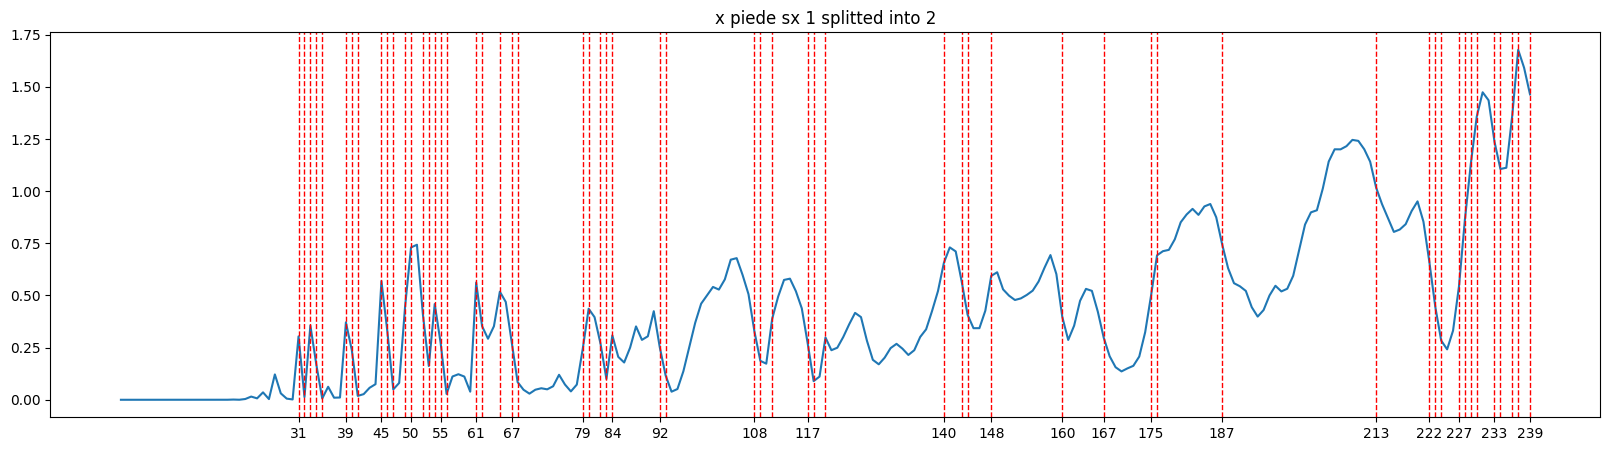
\includegraphics[width=0.8\linewidth,keepaspectratio]{x_piede_sx_1_008.png}
    \caption{Grafico degli errori per ogni periodo relativo al piede sinitro posizione 1 del soggetto sano $8$.}
    \label{fig:x_piede_sx_1_008_m2}
\end{figure}
\begin{figure}[H]
    \centering
    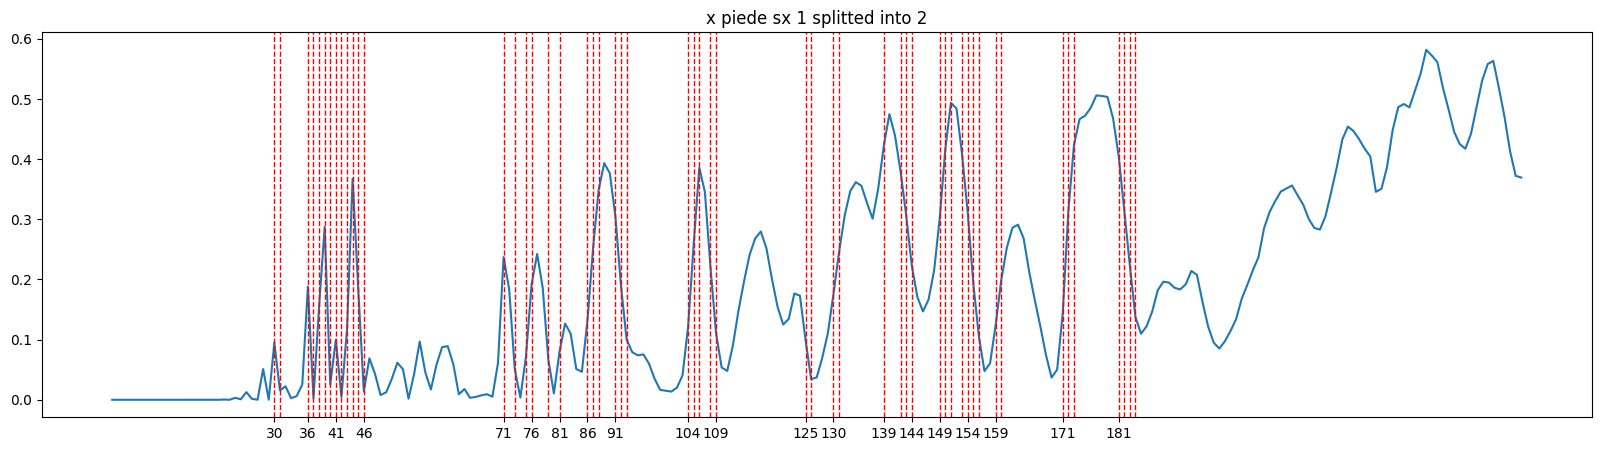
\includegraphics[width=0.8\linewidth,keepaspectratio]{x_piede_sx_1_021.png}
    \caption{Grafico degli errori per ogni periodo relativo al piede sinitro posizione 1 del soggetto patologico $21$.}
    \label{fig:x_piede_sx_1_021_m2}
\end{figure}

Nei grafici in figura~\ref*{fig:x_piede_sx_1_006_m2},~\ref*{fig:x_piede_sx_1_008_m2} e~\ref*{fig:x_piede_sx_1_021_m2}
sono rappresentati gli errori sull'asse delle ordinate ed i periodi, a cui ogni errore è associato,
sull'asse delle ascisse. Le linee rosse verticali rappresentano i punti salienti, calcolate mediante
l'asulio di una funzione che utilizza la media e deviazione standard della differenza tra un errore 
e quello successivo.

Controllando diversi grafici si è potuto notato che, per molte serie, in prossimità del periodo 
relativo ad un passo (stride) l'errore inizia ad alzarsi, in questo modo dovrebbe essere possibile 
calcolare la durata di un passo.
Questo però non succede sempre, con alcune serie questo fenomeno non si manifesta o comunque
si manifesta ma non in corrispondenza del periodo legato ad un passo, rendendo quindi impossibile
reperire l'informazione necessaria.

Questo potrebbe essere causato dal fatto che la funzione di seasonal decompose ``aggiusta'' la componente
di residui per riuscire ad ottenere una periodicità nella componente di stagionalità.

Tenendo a mente le considerazioni fatte fino questo punto possiamo quindi considerare i risultati ottenuti,
e di conseguenza questa soluzione, come non validi, essendo che non si ha la sicurezza di poter
ottenere risultati coerenti per la ricerca dell'informazione interessata.



\subsection{Conclusioni Finali}
Prendendo in considerazione la prima soluzione, spiegata nella sezione precedente, possiamo concludere
che la funzione di autocorrelazione può essere utilizzata per la soluzione a problemi di questa tipologia,
più in particolare essa può essere utilizzata per trovare pattern e/o caratteristiche presenti nei dati, 
che dal grafico potrebbero non essere evidenti.

La seconda soluzione proposta invece non è stata utile allo scopo di trovare un singolo passo 
relativo ad un soggetto. Normalmente consideriamo azioni abituali, come ad esempio il passo,
come pattern, di un determinato periodo, che si ripetono nel tempo quando invece nella realtà non 
è così. 
Tuttavia, l'algoritmo presentato nella seconda soluzione, potrebbe essere utilizzato 
in altre applicazioni la cui necessità ricade sul trovare periodi in cui occorrono stagionalità simili 
appartenenti a serie temporali diverse, oppure esso potrebbe essere preso come spunto implementativo per la creazione di un ulteriore 
algoritmo.

In conclusione, possiamo constatare che le tecniche utilizzate per l'analisi di serie temporali
possono essere d'aiuto per una prima analisi non accurata del problema,
non sostituendo però le tecniche tuttora utilizzate per analisi a problemi di questa tipologia.




    
    % bibliografia
    \section{Bibliografia}
    \printbibliography[title=Bibliografia]

    
\end{document}  